\documentclass[11pt,a4paper]{article}
\usepackage{lmodern}

\usepackage{amssymb,amsmath}
\usepackage{ifxetex,ifluatex}
\usepackage{fixltx2e} % provides \textsubscript
\ifnum 0\ifxetex 1\fi\ifluatex 1\fi=0 % if pdftex
  \usepackage[T1]{fontenc}
  \usepackage[utf8]{inputenc}
\else % if luatex or xelatex
  \ifxetex
    \usepackage{mathspec}
    \usepackage{xltxtra,xunicode}
  \else
    \usepackage{fontspec}
  \fi
  \defaultfontfeatures{Mapping=tex-text,Scale=MatchLowercase}
  \newcommand{\euro}{€}
\fi
% use upquote if available, for straight quotes in verbatim environments
\IfFileExists{upquote.sty}{\usepackage{upquote}}{}
% use microtype if available
\IfFileExists{microtype.sty}{%
\usepackage{microtype}
\UseMicrotypeSet[protrusion]{basicmath} % disable protrusion for tt fonts
}{}
\usepackage[lmargin=2.5cm,rmargin=2.5cm,tmargin=2.5cm,bmargin=2.5cm]{geometry}

% Figure Placement:
\usepackage{float}
\let\origfigure\figure
\let\endorigfigure\endfigure
\renewenvironment{figure}[1][2] {
    \expandafter\origfigure\expandafter[H]
} {
    \endorigfigure
}

%% citation setup

\usepackage{csquotes}

\usepackage[backend=biber, maxbibnames = 99, style = apa]{biblatex}
\setlength\bibitemsep{1.5\itemsep}
\bibliography{references.bib}
\usepackage{color}
\usepackage{fancyvrb}
\newcommand{\VerbBar}{|}
\newcommand{\VERB}{\Verb[commandchars=\\\{\}]}
\DefineVerbatimEnvironment{Highlighting}{Verbatim}{commandchars=\\\{\}}
% Add ',fontsize=\small' for more characters per line
\usepackage{framed}
\definecolor{shadecolor}{RGB}{248,248,248}
\newenvironment{Shaded}{\begin{snugshade}}{\end{snugshade}}
\newcommand{\AlertTok}[1]{\textcolor[rgb]{0.94,0.16,0.16}{#1}}
\newcommand{\AnnotationTok}[1]{\textcolor[rgb]{0.56,0.35,0.01}{\textbf{\textit{#1}}}}
\newcommand{\AttributeTok}[1]{\textcolor[rgb]{0.77,0.63,0.00}{#1}}
\newcommand{\BaseNTok}[1]{\textcolor[rgb]{0.00,0.00,0.81}{#1}}
\newcommand{\BuiltInTok}[1]{#1}
\newcommand{\CharTok}[1]{\textcolor[rgb]{0.31,0.60,0.02}{#1}}
\newcommand{\CommentTok}[1]{\textcolor[rgb]{0.56,0.35,0.01}{\textit{#1}}}
\newcommand{\CommentVarTok}[1]{\textcolor[rgb]{0.56,0.35,0.01}{\textbf{\textit{#1}}}}
\newcommand{\ConstantTok}[1]{\textcolor[rgb]{0.00,0.00,0.00}{#1}}
\newcommand{\ControlFlowTok}[1]{\textcolor[rgb]{0.13,0.29,0.53}{\textbf{#1}}}
\newcommand{\DataTypeTok}[1]{\textcolor[rgb]{0.13,0.29,0.53}{#1}}
\newcommand{\DecValTok}[1]{\textcolor[rgb]{0.00,0.00,0.81}{#1}}
\newcommand{\DocumentationTok}[1]{\textcolor[rgb]{0.56,0.35,0.01}{\textbf{\textit{#1}}}}
\newcommand{\ErrorTok}[1]{\textcolor[rgb]{0.64,0.00,0.00}{\textbf{#1}}}
\newcommand{\ExtensionTok}[1]{#1}
\newcommand{\FloatTok}[1]{\textcolor[rgb]{0.00,0.00,0.81}{#1}}
\newcommand{\FunctionTok}[1]{\textcolor[rgb]{0.00,0.00,0.00}{#1}}
\newcommand{\ImportTok}[1]{#1}
\newcommand{\InformationTok}[1]{\textcolor[rgb]{0.56,0.35,0.01}{\textbf{\textit{#1}}}}
\newcommand{\KeywordTok}[1]{\textcolor[rgb]{0.13,0.29,0.53}{\textbf{#1}}}
\newcommand{\NormalTok}[1]{#1}
\newcommand{\OperatorTok}[1]{\textcolor[rgb]{0.81,0.36,0.00}{\textbf{#1}}}
\newcommand{\OtherTok}[1]{\textcolor[rgb]{0.56,0.35,0.01}{#1}}
\newcommand{\PreprocessorTok}[1]{\textcolor[rgb]{0.56,0.35,0.01}{\textit{#1}}}
\newcommand{\RegionMarkerTok}[1]{#1}
\newcommand{\SpecialCharTok}[1]{\textcolor[rgb]{0.00,0.00,0.00}{#1}}
\newcommand{\SpecialStringTok}[1]{\textcolor[rgb]{0.31,0.60,0.02}{#1}}
\newcommand{\StringTok}[1]{\textcolor[rgb]{0.31,0.60,0.02}{#1}}
\newcommand{\VariableTok}[1]{\textcolor[rgb]{0.00,0.00,0.00}{#1}}
\newcommand{\VerbatimStringTok}[1]{\textcolor[rgb]{0.31,0.60,0.02}{#1}}
\newcommand{\WarningTok}[1]{\textcolor[rgb]{0.56,0.35,0.01}{\textbf{\textit{#1}}}}
\usepackage{longtable,booktabs}
\usepackage{graphicx}
\makeatletter
\def\maxwidth{\ifdim\Gin@nat@width>\linewidth\linewidth\else\Gin@nat@width\fi}
\def\maxheight{\ifdim\Gin@nat@height>\textheight\textheight\else\Gin@nat@height\fi}
\makeatother
% Scale images if necessary, so that they will not overflow the page
% margins by default, and it is still possible to overwrite the defaults
% using explicit options in \includegraphics[width, height, ...]{}
\setkeys{Gin}{width=\maxwidth,height=\maxheight,keepaspectratio}
\ifxetex
  \usepackage[setpagesize=false, % page size defined by xetex
              unicode=false, % unicode breaks when used with xetex
              xetex]{hyperref}
\else
  \usepackage[unicode=true]{hyperref}
\fi
\hypersetup{breaklinks=true,
            bookmarks=true,
            pdfauthor={Alexander Langnau, Öcal Kaptan, Sunyoung Ji},
            pdftitle={A Functional Approach to (parallelised) Monte Carlo Simulation},
            colorlinks=true,
            citecolor=blue,
            urlcolor=blue,
            linkcolor=magenta,
            pdfborder={0 0 0}}
\urlstyle{same}  % don't use monospace font for urls
\setlength{\parindent}{0pt}
\setlength{\parskip}{6pt plus 2pt minus 1pt}
\setlength{\emergencystretch}{3em}  % prevent overfull lines
\setcounter{secnumdepth}{5}

%%% Use protect on footnotes to avoid problems with footnotes in titles
\let\rmarkdownfootnote\footnote%
\def\footnote{\protect\rmarkdownfootnote}

%%% Change title format to be more compact
\usepackage{titling}

% Create subtitle command for use in maketitle
\newcommand{\subtitle}[1]{
  \posttitle{
    \begin{center}\large#1\end{center}
    }
}

\setlength{\droptitle}{-2em}
  \title{A Functional Approach to (parallelised) Monte Carlo Simulation}
  \pretitle{\vspace{\droptitle}\centering\huge}
  \posttitle{\par}
\subtitle{Advanced R for Econometricians}
  \author{Alexander Langnau, Öcal Kaptan, Sunyoung Ji}
  \preauthor{\centering\large\emph}
  \postauthor{\par}
  \predate{\centering\large\emph}
  \postdate{\par}
  \date{today}


%% linespread settings

\usepackage{setspace}

\onehalfspacing

% Language Setup

\usepackage{ifthen}
\usepackage{iflang}
\usepackage[super]{nth}

\ifthenelse{\equal{english}{german}}{
  \usepackage[ngerman]{babel}
  }{
  \usepackage[english]{babel}
  }

\begin{document}

\newgeometry{left=2cm,right=1cm,bottom=2cm,top=2cm}

\begin{titlepage}
  \noindent\begin{minipage}{0.6\textwidth}
	  \IfLanguageName{english}{University of Duisburg-Essen}{Universität Duisburg-Essen}\\
	  \IfLanguageName{english}{Faculty of Business Administration and Economics}{Fakultät für Wirtschaftswissensschaften}\\
	  \IfLanguageName{english}{Chair of Econometrics}{Lehrstuhl für Ökonometrie}\\
  \end{minipage}
	\begin{minipage}{0.4\textwidth}
	  \begin{flushright}
  	  \vspace{-0.5cm}
      \IfLanguageName{english}{\includegraphics*[width=5cm]{Includes/duelogo_en.png}}{\includegraphics*[width=5cm]{Includes/duelogo_de.png}}
	  \end{flushright}
	\end{minipage}
  \\
  \vspace{1.5cm}
  \begin{center}
  \huge{A Functional Approach to (parallelised) Monte Carlo
Simulation}\\
  \vspace{.25cm}
  \Large{Advanced R for Econometricians}\\
  \vspace{0.5cm}
  \large{Final Project}\\
  \vspace{1cm}
  \large{
  \IfLanguageName{english}{Submitted to the Faculty of \\ Business Administration and Economics \\at the \\University of Duisburg-Essen}{Vorgelegt der \\Fakultät für Wirtschaftswissenschaften der \\ Universität Duisburg-Essen}\\}
  \vspace{0.75cm}
  \large{\IfLanguageName{english}{from:}{von:}}\\
  \vspace{0.5cm}
  Alexander Langnau, Öcal Kaptan, Sunyoung Ji\\
  \end{center}
  \vspace{4cm}

  \noindent\begin{minipage}[t]{0.5\textwidth}
  \IfLanguageName{english}{Matriculation Number:}{Matrikelnummer}
  \end{minipage}
  \begin{minipage}[t]{0.7\textwidth}
  \hspace{1cm}232907, 230914, 229979
  \end{minipage}

  \noindent\begin{minipage}[t]{0.5\textwidth}
  \IfLanguageName{english}{Study Path:}{Studienfach:}
  \end{minipage}
  \begin{minipage}[t]{0.7\textwidth}
  \hspace{1cm}M.Sc. Econometrics
  \end{minipage}

  \noindent\begin{minipage}[t]{0.5\textwidth}
  \IfLanguageName{english}{Reviewer:}{Erstgutachter:}
  \end{minipage}
  \begin{minipage}[t]{0.7\textwidth}
  \hspace{1cm}Prof.~Dr.~Christoph Hanck
  \end{minipage}

  \noindent\begin{minipage}[t]{0.5\textwidth}
  \IfLanguageName{english}{Secondary Reviewer:}{Zweitgutachter}
  \end{minipage}
  \begin{minipage}[t]{0.7\textwidth}
  \hspace{1cm}M.Sc. Martin C. Arnold, M.Sc. Jens Klenke
  \end{minipage}

  \noindent\begin{minipage}[t]{0.5\textwidth}
  Semester:
  \end{minipage}
  \begin{minipage}[t]{0.7\textwidth}
  \hspace{1cm}\IfLanguageName{english}{\nth{1} Semester}{1. Fachsemester}
  \end{minipage}

  \noindent\begin{minipage}[t]{0.5\textwidth}
  \IfLanguageName{english}{Graduation (est.):}{Vsl. Studienabschluss:}
  \end{minipage}
  \begin{minipage}[t]{0.7\textwidth}
  \hspace{1cm}Summer Term 2022
  \end{minipage}

  \noindent\begin{minipage}[t]{0.5\textwidth}
  \IfLanguageName{english}{Deadline:}{Abgabefrist:}
  \end{minipage}
  \begin{minipage}[t]{0.7\textwidth}
  \hspace{1cm}09. 09. 2022
  \end{minipage}

\end{titlepage}

% Ends the declared geometry for the titlepage
\restoregeometry


\pagenumbering{Roman} 
{
\hypersetup{linkcolor=black}
\setcounter{tocdepth}{3}
\tableofcontents
}
\newpage
\listoftables
\newpage
\listoffigures
\newpage
\pagenumbering{arabic} 
\hypertarget{introduction}{%
\section{Introduction}\label{introduction}}

The Monte Carlo method is a simulation method for calculating the
probabilistic value of the desired function using random numbers. A
repeated pseudo-random number generator estimates sample statistics and
returns a probability distribution of the sample, representing the
parameter \autocite{Barbu_2020}. Monte Carlo methods are combined with
programming in modern research and contribute to various studies in
statistics, economics and many other scientific fields. This paper
progresses on developing a collection of different wrapper functions to
partially automatize the process of running a Monte Carlo simulation.
The Main function provides a convenient interface for Monte Carlo
simulations and allows user to create a parameter grid and iterate
homogeneous function calls over the parameter grid. It also offers
informative summary statistics, including visualization with
ggplot2-methods and an option to use a parallelisation plan using the
\texttt{furrr} package. The paper proceeds as follows: Chapter 2
describes pre-processes to establish the Monte Carlo simulation
function. The pre-process contain functions to create a parameter grid
and the respective data points drawn from a user-defined distribution,
along with functions that provide summary statistics. Chapter 3 details
the main Monte Carlo simulation function, which consists of the helper
functions introduced in chapter 2. Chapter 4 presents specific examples
for the simulation process. Finally, chapter 5 summarizes the work
presented in this paper. Concerning the size of the main function
result, the outputs of the simulation results in chapter 4 reported in
Appendix.

\hypertarget{pre-process-creating-helper-functions}{%
\section{Pre-process: Creating Helper
functions}\label{pre-process-creating-helper-functions}}

The pre-process comprises 5 helper functions: \texttt{create\_grid()},
\texttt{data\_generation()}, \texttt{summary\_function()},
\texttt{create\_array\_function()} and \texttt{output\_function()}. The
functions are named in a way that the underlying purpose is directly
clear. These functions are the building blocks of the
\texttt{main\_function()}, which takes the user input and runs the Monte
Carlo simulation by itself.

\hypertarget{create_grid}{%
\subsection{create\_grid()}\label{create_grid}}

The first helper function introduced is the
\texttt{create\_grid()}-function, which automatically creates a
hyper-parameter grid over all permutations specified by the user.

\begin{Shaded}
\begin{Highlighting}[]
\NormalTok{create\_grid }\OtherTok{\textless{}{-}} \ControlFlowTok{function}\NormalTok{(parameters, nrep)\{}
\NormalTok{  input }\OtherTok{\textless{}{-}}\NormalTok{ parameters}
\NormalTok{  storage }\OtherTok{\textless{}{-}} \FunctionTok{list}\NormalTok{()}
\NormalTok{  name\_vec }\OtherTok{\textless{}{-}} \FunctionTok{c}\NormalTok{()}
  
  \ControlFlowTok{for}\NormalTok{(i }\ControlFlowTok{in} \DecValTok{1}\SpecialCharTok{:}\FunctionTok{length}\NormalTok{(input))\{ }\CommentTok{\#1:3}
\NormalTok{    a }\OtherTok{\textless{}{-}} \FunctionTok{as.numeric}\NormalTok{(input[[i]][[}\DecValTok{2}\NormalTok{]])}
\NormalTok{    b }\OtherTok{\textless{}{-}} \FunctionTok{as.numeric}\NormalTok{(input[[i]][[}\DecValTok{3}\NormalTok{]])}
\NormalTok{    c }\OtherTok{\textless{}{-}} \FunctionTok{as.numeric}\NormalTok{(input[[i]][[}\DecValTok{4}\NormalTok{]])}
\NormalTok{    output }\OtherTok{\textless{}{-}} \FunctionTok{seq}\NormalTok{(}\AttributeTok{from=}\NormalTok{a, }\AttributeTok{to=}\NormalTok{b, }\AttributeTok{by=}\NormalTok{c)}
\NormalTok{    storage[[i]] }\OtherTok{\textless{}{-}}\NormalTok{  output}
\NormalTok{    name\_vec[i] }\OtherTok{\textless{}{-}}\NormalTok{ input[[i]][[}\DecValTok{1}\NormalTok{]]}
\NormalTok{  \}}
  
\NormalTok{  grid }\OtherTok{\textless{}{-}} \FunctionTok{expand\_grid}\NormalTok{(}\FunctionTok{unlist}\NormalTok{(storage[}\DecValTok{1}\NormalTok{])}
\NormalTok{                      , }\FunctionTok{unlist}\NormalTok{(storage[}\DecValTok{2}\NormalTok{])}
\NormalTok{                      , }\FunctionTok{unlist}\NormalTok{(storage[}\DecValTok{3}\NormalTok{])}
\NormalTok{                      , }\FunctionTok{unlist}\NormalTok{(storage[}\DecValTok{4}\NormalTok{])}
\NormalTok{                      , }\FunctionTok{unlist}\NormalTok{(storage[}\DecValTok{5}\NormalTok{])}
\NormalTok{                      , }\FunctionTok{c}\NormalTok{(}\DecValTok{1}\SpecialCharTok{:}\NormalTok{nrep))}
  
  \FunctionTok{names}\NormalTok{(grid) }\OtherTok{\textless{}{-}} \FunctionTok{c}\NormalTok{(name\_vec, }\StringTok{"rep"}\NormalTok{)}
  
  \FunctionTok{return}\NormalTok{(grid)}
\NormalTok{\}}
\end{Highlighting}
\end{Shaded}

Input for the parameter list has to follow a specific format as shown
below:

\begin{verbatim}
parameter_list <- list(c("variable name 1", from, to, by) 
                      ,c("variable name 2", from, to, by)
                      ,c("variable name 3", from, to, by)
                      ,c("variable name 4", from, to, by))
\end{verbatim}

\texttt{parameter\_list} works with a minimum of 1 and a maximum of 4
variables. The structure of arguments is similar to \texttt{seq()} in R:
Each vector contained in the list needs four arguments specified, that
is, the function name, the start of the sequence, the end of the
sequence and the steps, by which the interval gets divided. It would be
easy to adapt this helper function for more parameters, but it is
assumed that a grid with up to 4 parameters offers enough complexity for
the simulation. The function basically takes the information of the
input parameter list and creates a grid with
\texttt{tidyr::expand\_grid()}. The argument \texttt{nrep} specifies how
many repetitions per parameter constellation are created, where a
separate row in the parameter grid gets created for each repetition.

\textbf{Example to \texttt{create\_grid()}:}

\begin{Shaded}
\begin{Highlighting}[]
\CommentTok{\#four parameters }
\NormalTok{param\_list0 }\OtherTok{\textless{}{-}} \FunctionTok{list}\NormalTok{(}\FunctionTok{c}\NormalTok{(}\StringTok{"n"}\NormalTok{, }\DecValTok{10}\NormalTok{, }\DecValTok{20}\NormalTok{, }\DecValTok{10}\NormalTok{)}
\NormalTok{                    ,}\FunctionTok{c}\NormalTok{(}\StringTok{"mu"}\NormalTok{, }\DecValTok{0}\NormalTok{, }\FloatTok{0.5}\NormalTok{, }\FloatTok{0.25}\NormalTok{)}
\NormalTok{                    ,}\FunctionTok{c}\NormalTok{(}\StringTok{"sd"}\NormalTok{, }\DecValTok{0}\NormalTok{, }\FloatTok{0.3}\NormalTok{, }\FloatTok{0.1}\NormalTok{)}
\NormalTok{                    ,}\FunctionTok{c}\NormalTok{(}\StringTok{"gender"}\NormalTok{, }\DecValTok{0}\NormalTok{, }\DecValTok{1}\NormalTok{, }\DecValTok{1}\NormalTok{))}

\FunctionTok{head}\NormalTok{(}\FunctionTok{create\_grid}\NormalTok{(param\_list0, }\AttributeTok{nrep=}\DecValTok{3}\NormalTok{), }\AttributeTok{n=}\DecValTok{10}\NormalTok{)}
\end{Highlighting}
\end{Shaded}

\begin{verbatim}
## # A tibble: 10 x 5
##        n    mu    sd gender   rep
##    <dbl> <dbl> <dbl>  <dbl> <int>
##  1    10     0   0        0     1
##  2    10     0   0        0     2
##  3    10     0   0        0     3
##  4    10     0   0        1     1
##  5    10     0   0        1     2
##  6    10     0   0        1     3
##  7    10     0   0.1      0     1
##  8    10     0   0.1      0     2
##  9    10     0   0.1      0     3
## 10    10     0   0.1      1     1
\end{verbatim}

\hypertarget{data_generation}{%
\subsection{data\_generation()}\label{data_generation}}

The second helper function called \texttt{data\_generation()} takes the
arguments \texttt{grid} and \texttt{simulation} as inputs.
\texttt{simulation} is the argument for the user-defined function for
the data generation process, while \texttt{grid} is the parameter grid
previously created. The user can choose between a variety of probability
distributions by entering the name of the function, for example,
\texttt{rnorm()} for the normal distribution or \texttt{runif()} for the
uniform distribution.

The n data points created for each set of parameters are stored as
separate elements in a list since this format is a very flexible way of
storing data.

\texttt{data\_generation()} chooses relative mapping function base on
specification shown as on the table below.

\begin{longtable}[]{@{}ccc@{}}
\toprule()
Mapping & Mapping with parallelisation & Number of parameters \\
\midrule()
\endhead
\texttt{purrr:map()} & \texttt{furrrr:future\_map()} & \(n = 1\) \\
\texttt{purrr:map2()} & \texttt{furrrr:future\_map2()} & \(n = 2\) \\
\texttt{purrr:pmap()} & \texttt{furrrr:future\_pmap()} & \(n \geq 3\) \\
\bottomrule()
\end{longtable}

\texttt{options\ =\ furrr\_options(seed\ =\ TRUE)} is for reproducible
random number generation (RNG) processes. This argument takes control of
the RNG process for parallelization and always generates the same
numbers according to the given seed. More details can be found by
running the command \texttt{?furrr\_options} in RStudio.

\begin{Shaded}
\begin{Highlighting}[]
\NormalTok{data\_generation }\OtherTok{\textless{}{-}} \ControlFlowTok{function}\NormalTok{(simulation, grid)\{}
  
  \ControlFlowTok{if}\NormalTok{(}\FunctionTok{ncol}\NormalTok{(grid)}\SpecialCharTok{==}\DecValTok{2}\NormalTok{)\{}
\NormalTok{    var1 }\OtherTok{\textless{}{-}} \FunctionTok{c}\NormalTok{(}\FunctionTok{unlist}\NormalTok{(grid[,}\DecValTok{1}\NormalTok{]))}
    \ControlFlowTok{if}\NormalTok{(cores}\SpecialCharTok{\textgreater{}}\DecValTok{1}\NormalTok{)\{}
\NormalTok{      data }\OtherTok{\textless{}{-}} \FunctionTok{future\_map}\NormalTok{(var1, simulation,}
                         \AttributeTok{.options =} \FunctionTok{furrr\_options}\NormalTok{(}\AttributeTok{seed =} \ConstantTok{TRUE}\NormalTok{))}
\NormalTok{    \}}\ControlFlowTok{else}\NormalTok{\{}
\NormalTok{      data }\OtherTok{\textless{}{-}} \FunctionTok{map}\NormalTok{(var1, simulation)}
\NormalTok{    \}}
\NormalTok{  \}}
  
  \ControlFlowTok{if}\NormalTok{(}\FunctionTok{ncol}\NormalTok{(grid)}\SpecialCharTok{==}\DecValTok{3}\NormalTok{)\{}
\NormalTok{    var1 }\OtherTok{\textless{}{-}} \FunctionTok{c}\NormalTok{(}\FunctionTok{unlist}\NormalTok{(grid[,}\DecValTok{1}\NormalTok{]))}
\NormalTok{    var2 }\OtherTok{\textless{}{-}} \FunctionTok{c}\NormalTok{(}\FunctionTok{unlist}\NormalTok{(grid[,}\DecValTok{2}\NormalTok{]))}
    \ControlFlowTok{if}\NormalTok{(cores}\SpecialCharTok{\textgreater{}}\DecValTok{1}\NormalTok{)\{}
\NormalTok{      data }\OtherTok{\textless{}{-}} \FunctionTok{future\_map2}\NormalTok{(var1, var2, simulation,}
                          \AttributeTok{.options =} \FunctionTok{furrr\_options}\NormalTok{(}\AttributeTok{seed =} \ConstantTok{TRUE}\NormalTok{))}
\NormalTok{    \} }\ControlFlowTok{else}\NormalTok{\{}
\NormalTok{      data }\OtherTok{\textless{}{-}} \FunctionTok{map2}\NormalTok{(var1, var2, simulation)}
\NormalTok{    \}}
\NormalTok{  \} }
  
  \ControlFlowTok{if}\NormalTok{(}\FunctionTok{ncol}\NormalTok{(grid)}\SpecialCharTok{==}\DecValTok{4}\NormalTok{)\{}
\NormalTok{    var1 }\OtherTok{\textless{}{-}} \FunctionTok{c}\NormalTok{(}\FunctionTok{unlist}\NormalTok{(grid[,}\DecValTok{1}\NormalTok{]))}
\NormalTok{    var2 }\OtherTok{\textless{}{-}} \FunctionTok{c}\NormalTok{(}\FunctionTok{unlist}\NormalTok{(grid[,}\DecValTok{2}\NormalTok{]))}
\NormalTok{    var3 }\OtherTok{\textless{}{-}} \FunctionTok{c}\NormalTok{(}\FunctionTok{unlist}\NormalTok{(grid[,}\DecValTok{3}\NormalTok{]))}
\NormalTok{    list1 }\OtherTok{\textless{}{-}} \FunctionTok{list}\NormalTok{(var1,var2,var3)}
    \ControlFlowTok{if}\NormalTok{(cores}\SpecialCharTok{\textgreater{}}\DecValTok{1}\NormalTok{)\{}
\NormalTok{      data }\OtherTok{\textless{}{-}} \FunctionTok{future\_pmap}\NormalTok{(list1, }\AttributeTok{.f=}\NormalTok{simulation,}
                          \AttributeTok{.options =} \FunctionTok{furrr\_options}\NormalTok{(}\AttributeTok{seed =} \ConstantTok{TRUE}\NormalTok{))}
\NormalTok{    \}}\ControlFlowTok{else}\NormalTok{\{}
\NormalTok{      data }\OtherTok{\textless{}{-}} \FunctionTok{pmap}\NormalTok{(list1, }\AttributeTok{.f=}\NormalTok{simulation)}
\NormalTok{    \}}
\NormalTok{  \}}
  
  \FunctionTok{return}\NormalTok{(data)}
\NormalTok{\}}
\end{Highlighting}
\end{Shaded}

Monte Carlo simulations can become very demanding in terms of computing
time. In that case, parallel processing may be used to reduce the time
of the simulation. In parallel processes, each process is executed
simultaneously but independently. Interconnections are proceeded through
communication channel \autocite{Czech_2017}.

\texttt{data\_generation()} automatically used the proper function from
the \texttt{furrrr}-package. If the user specified more than one core.
Otherwise, the function will stick to the respective mapping function
from the \texttt{purrr}-package.

\textbf{Example to \texttt{data\_generation()}:} The example below
demonstrates the data generation process with Poisson distribution
without parallelisation. The advantage in computation time with
parallelisation will be discussed in Chapter 3.

\begin{Shaded}
\begin{Highlighting}[]
\NormalTok{cores }\OtherTok{\textless{}{-}} \DecValTok{1}


\NormalTok{param\_list2 }\OtherTok{\textless{}{-}} \FunctionTok{list}\NormalTok{(}\FunctionTok{c}\NormalTok{(}\StringTok{"n"}\NormalTok{, }\DecValTok{10}\NormalTok{, }\DecValTok{20}\NormalTok{, }\DecValTok{10}\NormalTok{)}
\NormalTok{                  ,}\FunctionTok{c}\NormalTok{(}\StringTok{"lambda"}\NormalTok{, }\FloatTok{0.5}\NormalTok{, }\DecValTok{1}\NormalTok{, }\FloatTok{0.5}\NormalTok{))}



\NormalTok{grid2 }\OtherTok{\textless{}{-}} \FunctionTok{create\_grid}\NormalTok{(param\_list2, }\AttributeTok{nrep=}\DecValTok{1}\NormalTok{)}
\NormalTok{sim1 }\OtherTok{\textless{}{-}} \FunctionTok{data\_generation}\NormalTok{(}\AttributeTok{simulation=}\NormalTok{rpois, }\AttributeTok{grid=}\NormalTok{grid2)}


\FunctionTok{names}\NormalTok{(sim1) }\OtherTok{\textless{}{-}} \FunctionTok{c}\NormalTok{(}\StringTok{"n=10, lamda = 0.5"}\NormalTok{,}\StringTok{"n=10, lamda = 1"}\NormalTok{,}
                 \StringTok{"n=20, lamda = 0.5"}\NormalTok{,}\StringTok{"n=20, lamda = 1"}\NormalTok{)}
\NormalTok{grid2}
\end{Highlighting}
\end{Shaded}

\begin{verbatim}
## # A tibble: 4 x 3
##       n lambda   rep
##   <dbl>  <dbl> <int>
## 1    10    0.5     1
## 2    10    1       1
## 3    20    0.5     1
## 4    20    1       1
\end{verbatim}

\begin{Shaded}
\begin{Highlighting}[]
\NormalTok{sim1}
\end{Highlighting}
\end{Shaded}

\begin{verbatim}
## $`n=10, lamda = 0.5`
##  [1] 0 1 0 1 2 0 0 1 0 0
## 
## $`n=10, lamda = 1`
##  [1] 3 1 1 1 0 2 0 0 0 3
## 
## $`n=20, lamda = 0.5`
##  [1] 1 1 1 3 1 1 0 0 0 0 2 1 1 1 0 0 1 0 0 0
## 
## $`n=20, lamda = 1`
##  [1] 0 1 1 1 0 0 0 1 0 2 0 1 2 0 1 0 0 2 2 1
\end{verbatim}

\texttt{sim1} contains the generated data by \texttt{data\_generation()}
with \texttt{grid2} and Poisson distribution as input. The function
below shows the application of \texttt{data\_generation()} to uniform
and Poisson distribution:

\begin{Shaded}
\begin{Highlighting}[]
\CommentTok{\# Application to uniform distribution}
\NormalTok{param\_list\_runif }\OtherTok{\textless{}{-}} \FunctionTok{list}\NormalTok{(}\FunctionTok{c}\NormalTok{(}\StringTok{"n"}\NormalTok{, }\DecValTok{10}\NormalTok{, }\DecValTok{30}\NormalTok{, }\DecValTok{10}\NormalTok{)}
\NormalTok{                         ,}\FunctionTok{c}\NormalTok{(}\StringTok{"min"}\NormalTok{, }\DecValTok{0}\NormalTok{, }\DecValTok{0}\NormalTok{, }\DecValTok{0}\NormalTok{)}
\NormalTok{                         ,}\FunctionTok{c}\NormalTok{(}\StringTok{"max"}\NormalTok{, }\DecValTok{1}\NormalTok{, }\DecValTok{1}\NormalTok{, }\DecValTok{0}\NormalTok{))}


\NormalTok{grid\_unif }\OtherTok{\textless{}{-}} \FunctionTok{create\_grid}\NormalTok{(param\_list\_runif, }\AttributeTok{nrep=}\DecValTok{3}\NormalTok{)}
\FunctionTok{head}\NormalTok{(}\FunctionTok{data\_generation}\NormalTok{(}\AttributeTok{simulation=}\NormalTok{runif, }\AttributeTok{grid=}\NormalTok{grid\_unif),}\DecValTok{1}\NormalTok{)}
\end{Highlighting}
\end{Shaded}

\begin{verbatim}
## $n1
##  [1] 0.66511519 0.09484066 0.38396964 0.27438364 0.81464004 0.44851634
##  [7] 0.81006435 0.81238951 0.79434232 0.43983169
\end{verbatim}

As explained before, the data is stored in a list, where data points for
each set of parameters are stored under a different variable. The first
variable (saved under \texttt{\$n1}) is based on 10 draws from a uniform
distribution with \(\mathcal{U}_{[0,2]}\). Each variable in the list
relates to a row in the parameter grid.

\hypertarget{summary_function}{%
\subsection{summary\_function()}\label{summary_function}}

So far, the paper explains how to create \emph{raw} data with the
functions \texttt{create\_grid()} and \texttt{data\_generation()} using
chosen probability distribution. This chapter introduces
\texttt{summary\_function()} which applies a user-defined function to
create summary statistic on the raw data generated before. The function
uses a sapply-loop to apply the user-defined
summary\_function()(\texttt{sum\_fun})(such as mean()) on each element
of the list containing the raw data. Results are stored in a
\((nrow(grid ) X 1)\)-dimensional matrix, which is combined with the
parameter grid in the next step.

\begin{Shaded}
\begin{Highlighting}[]
\NormalTok{summary\_function }\OtherTok{\textless{}{-}} \ControlFlowTok{function}\NormalTok{(sum\_fun, data\_input)\{}
  
\NormalTok{  count }\OtherTok{\textless{}{-}} \FunctionTok{length}\NormalTok{(data\_input)}
\NormalTok{  summary\_matrix }\OtherTok{\textless{}{-}} \FunctionTok{matrix}\NormalTok{(}\AttributeTok{nrow=}\NormalTok{count, }\AttributeTok{ncol=}\DecValTok{1}\NormalTok{)}
  
  \ControlFlowTok{for}\NormalTok{(i }\ControlFlowTok{in} \DecValTok{1}\SpecialCharTok{:}\NormalTok{count)\{}
\NormalTok{    input }\OtherTok{\textless{}{-}} \FunctionTok{list}\NormalTok{(data\_input[[i]])}
\NormalTok{    output }\OtherTok{\textless{}{-}} \FunctionTok{sapply}\NormalTok{(sum\_fun, do.call, input)}
\NormalTok{    summary\_matrix[i] }\OtherTok{\textless{}{-}}\NormalTok{ output}
\NormalTok{  \}}

  \FunctionTok{colnames}\NormalTok{(summary\_matrix) }\OtherTok{\textless{}{-}}\NormalTok{ sum\_fun}
  \FunctionTok{return}\NormalTok{(summary\_matrix)}
\NormalTok{\}}
\end{Highlighting}
\end{Shaded}

\textbf{\texttt{summary\_function()} Example:}

For this example, data is generated using the normal distribution, with
the respective parameters n, \(\mu\) and \(\sigma\) specified in the
parameter list. The list containing the raw data created by
\texttt{data\_generation()} is stored in the variable
\texttt{test\_data}, which is the data input for
\texttt{summary\_function()}. The arithmetic mean, with base R
\texttt{mean()} function, is supplied as the second input to calculate
the mean of all the data points created under a unique set of
parameters. The output relates exactly to each row of the used parameter
grid. Later, these summary statistics R merged with the parameter grid
in a data frame.

\begin{Shaded}
\begin{Highlighting}[]
\NormalTok{param\_list3 }\OtherTok{\textless{}{-}} \FunctionTok{list}\NormalTok{(}\FunctionTok{c}\NormalTok{(}\StringTok{"n"}\NormalTok{, }\DecValTok{10}\NormalTok{, }\DecValTok{20}\NormalTok{, }\DecValTok{10}\NormalTok{)}
\NormalTok{                    ,}\FunctionTok{c}\NormalTok{(}\StringTok{"mu"}\NormalTok{, }\DecValTok{1}\NormalTok{, }\DecValTok{2}\NormalTok{, }\FloatTok{0.25}\NormalTok{)}
\NormalTok{                    ,}\FunctionTok{c}\NormalTok{(}\StringTok{"sd"}\NormalTok{, }\FloatTok{0.5}\NormalTok{, }\DecValTok{1}\NormalTok{, }\FloatTok{0.1}\NormalTok{))}

\NormalTok{grid\_test }\OtherTok{\textless{}{-}} \FunctionTok{create\_grid}\NormalTok{(param\_list3, }\AttributeTok{nrep=}\DecValTok{3}\NormalTok{)}
\NormalTok{test\_data }\OtherTok{\textless{}{-}} \FunctionTok{data\_generation}\NormalTok{(}\AttributeTok{simulation=}\NormalTok{rnorm, }\AttributeTok{grid=}\NormalTok{grid\_test)}
\NormalTok{summary\_data }\OtherTok{\textless{}{-}} \FunctionTok{summary\_function}\NormalTok{(}\AttributeTok{sum\_fun=}\FunctionTok{list}\NormalTok{(}\StringTok{"mean"}\NormalTok{),}
                                 \AttributeTok{data\_input=}\NormalTok{test\_data)}
\FunctionTok{head}\NormalTok{(summary\_data)}
\end{Highlighting}
\end{Shaded}

\begin{verbatim}
##           mean
## [1,] 0.9447809
## [2,] 1.0168699
## [3,] 0.7629786
## [4,] 1.0764221
## [5,] 1.1742643
## [6,] 1.0260035
\end{verbatim}

\begin{Shaded}
\begin{Highlighting}[]
\FunctionTok{nrow}\NormalTok{(summary\_data)}
\end{Highlighting}
\end{Shaded}

\begin{verbatim}
## [1] 180
\end{verbatim}

\hypertarget{create_array_function}{%
\subsection{create\_array\_function()}\label{create_array_function}}

?????????????Even though the example above includes a relatively small
parameter grids, the simulation returns 180 summarize data points. In
\texttt{main\_function()}, the results from the previous step get merged
with the parameter grid into one data frame. This way of storing the
data allows user to apply further data wrangling processes. A
multidimensional array is more suitable for printing the output in a
tidy and clear way. \texttt{create\_array\_function()} takes all
relevant data from the previous steps (parameter grid and the results of
the Monte Carlo simulation) and transforms it into an array with the
correct dimensions.???????????????

\begin{Shaded}
\begin{Highlighting}[]
\NormalTok{create\_array\_function }\OtherTok{\textless{}{-}} \ControlFlowTok{function}\NormalTok{(comb, parameters, nrep)\{}
\NormalTok{  storage }\OtherTok{\textless{}{-}} \FunctionTok{list}\NormalTok{()}
\NormalTok{  name\_vec }\OtherTok{\textless{}{-}} \FunctionTok{c}\NormalTok{()}
  
  \ControlFlowTok{for}\NormalTok{(i }\ControlFlowTok{in} \DecValTok{1}\SpecialCharTok{:}\FunctionTok{length}\NormalTok{(parameters))\{ }
\NormalTok{    a }\OtherTok{\textless{}{-}} \FunctionTok{as.numeric}\NormalTok{(parameters[[i]][[}\DecValTok{2}\NormalTok{]])}
\NormalTok{    b }\OtherTok{\textless{}{-}} \FunctionTok{as.numeric}\NormalTok{(parameters[[i]][[}\DecValTok{3}\NormalTok{]])}
\NormalTok{    c }\OtherTok{\textless{}{-}} \FunctionTok{as.numeric}\NormalTok{(parameters[[i]][[}\DecValTok{4}\NormalTok{]])}
\NormalTok{    output }\OtherTok{\textless{}{-}} \FunctionTok{seq}\NormalTok{(}\AttributeTok{from=}\NormalTok{a, }\AttributeTok{to=}\NormalTok{b, }\AttributeTok{by=}\NormalTok{c)}
\NormalTok{    storage[[i]] }\OtherTok{\textless{}{-}}\NormalTok{  output}
\NormalTok{    name\_vec[i] }\OtherTok{\textless{}{-}}\NormalTok{ parameters[[i]][[}\DecValTok{1}\NormalTok{]] }
\NormalTok{  \}}
  
  
\NormalTok{  matrix.numeration }\OtherTok{\textless{}{-}}  \FunctionTok{paste}\NormalTok{(}\StringTok{"rep"}\NormalTok{,}\StringTok{"="}\NormalTok{, }\DecValTok{1}\SpecialCharTok{:}\NormalTok{nrep, }\AttributeTok{sep =} \StringTok{""}\NormalTok{)}
  
  \ControlFlowTok{if}\NormalTok{(}\FunctionTok{length}\NormalTok{(parameters)}\SpecialCharTok{==}\DecValTok{1}\NormalTok{)\{}
\NormalTok{    comb\_ordered }\OtherTok{\textless{}{-}}\NormalTok{  comb }\SpecialCharTok{\%\textgreater{}\%} \FunctionTok{arrange}\NormalTok{(comb[,}\DecValTok{2}\NormalTok{])}
\NormalTok{    seq1 }\OtherTok{\textless{}{-}} \FunctionTok{c}\NormalTok{(}\FunctionTok{unlist}\NormalTok{(storage[}\DecValTok{1}\NormalTok{]))}
    
\NormalTok{    row.names }\OtherTok{\textless{}{-}} \FunctionTok{paste}\NormalTok{(name\_vec[}\DecValTok{1}\NormalTok{],}\StringTok{"="}\NormalTok{,seq1, }\AttributeTok{sep =} \StringTok{""}\NormalTok{)}
    
\NormalTok{    dimension\_array }\OtherTok{\textless{}{-}} \FunctionTok{c}\NormalTok{(}\FunctionTok{length}\NormalTok{(seq1), nrep)}
\NormalTok{    dim\_names\_list }\OtherTok{\textless{}{-}} \FunctionTok{list}\NormalTok{(row.names, matrix.numeration)}
\NormalTok{  \}}
  
  \ControlFlowTok{if}\NormalTok{(}\FunctionTok{length}\NormalTok{(parameters)}\SpecialCharTok{==}\DecValTok{2}\NormalTok{)\{}
\NormalTok{    comb\_ordered }\OtherTok{\textless{}{-}}\NormalTok{  comb }\SpecialCharTok{\%\textgreater{}\%} \FunctionTok{arrange}\NormalTok{(comb[,}\DecValTok{2}\NormalTok{])  }\SpecialCharTok{\%\textgreater{}\%} \FunctionTok{arrange}\NormalTok{(comb[,}\DecValTok{3}\NormalTok{])}
\NormalTok{    seq1 }\OtherTok{\textless{}{-}} \FunctionTok{c}\NormalTok{(}\FunctionTok{unlist}\NormalTok{(storage[}\DecValTok{1}\NormalTok{]))}
\NormalTok{    seq2 }\OtherTok{\textless{}{-}} \FunctionTok{c}\NormalTok{(}\FunctionTok{unlist}\NormalTok{(storage[}\DecValTok{2}\NormalTok{]))}
    
\NormalTok{    row.names }\OtherTok{\textless{}{-}} \FunctionTok{paste}\NormalTok{(name\_vec[}\DecValTok{1}\NormalTok{],}\StringTok{"="}\NormalTok{,seq1, }\AttributeTok{sep =} \StringTok{""}\NormalTok{)}
\NormalTok{    column.names }\OtherTok{\textless{}{-}}  \FunctionTok{paste}\NormalTok{(name\_vec[}\DecValTok{2}\NormalTok{],}\StringTok{"="}\NormalTok{,seq2, }\AttributeTok{sep =} \StringTok{""}\NormalTok{)}
    
\NormalTok{    dimension\_array }\OtherTok{\textless{}{-}} \FunctionTok{c}\NormalTok{(}\FunctionTok{length}\NormalTok{(seq1), }\FunctionTok{length}\NormalTok{(seq2), nrep)}
\NormalTok{    dim\_names\_list }\OtherTok{\textless{}{-}} \FunctionTok{list}\NormalTok{(row.names, column.names, matrix.numeration)}
\NormalTok{  \}}
  
  \ControlFlowTok{if}\NormalTok{(}\FunctionTok{length}\NormalTok{(parameters)}\SpecialCharTok{==}\DecValTok{3}\NormalTok{)\{}
\NormalTok{    comb\_ordered }\OtherTok{\textless{}{-}}\NormalTok{  comb }\SpecialCharTok{\%\textgreater{}\%} \FunctionTok{arrange}\NormalTok{(comb[,}\DecValTok{2}\NormalTok{])  }\SpecialCharTok{\%\textgreater{}\%} 
      \FunctionTok{arrange}\NormalTok{(comb[,}\DecValTok{3}\NormalTok{]) }\SpecialCharTok{\%\textgreater{}\%} \FunctionTok{arrange}\NormalTok{(comb[,}\DecValTok{4}\NormalTok{]) }
\NormalTok{    seq1 }\OtherTok{\textless{}{-}} \FunctionTok{c}\NormalTok{(}\FunctionTok{unlist}\NormalTok{(storage[}\DecValTok{1}\NormalTok{]))}
\NormalTok{    seq2 }\OtherTok{\textless{}{-}} \FunctionTok{c}\NormalTok{(}\FunctionTok{unlist}\NormalTok{(storage[}\DecValTok{2}\NormalTok{]))}
\NormalTok{    seq3 }\OtherTok{\textless{}{-}} \FunctionTok{c}\NormalTok{(}\FunctionTok{unlist}\NormalTok{(storage[}\DecValTok{3}\NormalTok{]))}
    
\NormalTok{    row.names }\OtherTok{\textless{}{-}} \FunctionTok{paste}\NormalTok{(name\_vec[}\DecValTok{1}\NormalTok{],}\StringTok{"="}\NormalTok{,seq1, }\AttributeTok{sep =} \StringTok{""}\NormalTok{)}
\NormalTok{    column.names }\OtherTok{\textless{}{-}}  \FunctionTok{paste}\NormalTok{(name\_vec[}\DecValTok{2}\NormalTok{],}\StringTok{"="}\NormalTok{,seq2, }\AttributeTok{sep =} \StringTok{""}\NormalTok{)}
\NormalTok{    matrix.names1 }\OtherTok{\textless{}{-}}  \FunctionTok{paste}\NormalTok{(name\_vec[}\DecValTok{3}\NormalTok{],}\StringTok{"="}\NormalTok{,seq3, }\AttributeTok{sep =} \StringTok{""}\NormalTok{)}
    
\NormalTok{    dimension\_array }\OtherTok{\textless{}{-}} \FunctionTok{c}\NormalTok{(}\FunctionTok{length}\NormalTok{(seq1), }\FunctionTok{length}\NormalTok{(seq2), }\FunctionTok{length}\NormalTok{(seq3), nrep)}
\NormalTok{    dim\_names\_list }\OtherTok{\textless{}{-}} \FunctionTok{list}\NormalTok{(row.names, column.names, }
\NormalTok{                           matrix.names1, matrix.numeration)}
    
\NormalTok{  \}}
  
  
\NormalTok{  array1 }\OtherTok{\textless{}{-}} \FunctionTok{array}\NormalTok{(comb\_ordered[,}\FunctionTok{ncol}\NormalTok{(comb)] }
\NormalTok{                  , }\AttributeTok{dim =}\NormalTok{ dimension\_array}
\NormalTok{                  , dim\_names\_list)}
  \FunctionTok{return}\NormalTok{(array1)}
\NormalTok{\}}
\end{Highlighting}
\end{Shaded}

In order to test \texttt{create\_array\_function()}, we need to set up
an altered version of \texttt{main\_function()}. The
\texttt{main\_function()} is discussed in the next chapter. Also, a
slightly modified version of the example using the \texttt{rnorm()} is
used, where the parameter grid spans over a larger sequence

\textbf{Example to \texttt{create\_array\_function} :}

\begin{Shaded}
\begin{Highlighting}[]
\CommentTok{\# PREP }\AlertTok{TEST}\CommentTok{ \textasciigrave{}create\_array\_function\textasciigrave{}}
\NormalTok{main\_function\_array\_test }\OtherTok{\textless{}{-}}  \ControlFlowTok{function}\NormalTok{(parameters }\CommentTok{\#list of parameters}
\NormalTok{                                      , nrep }\CommentTok{\#number of repetitions}
\NormalTok{                                      , simulation }\CommentTok{\#data genereation}
\NormalTok{                                      , sum\_fun)\{ }\CommentTok{\#summary statistics}
  
\NormalTok{  grid }\OtherTok{\textless{}{-}} \FunctionTok{create\_grid}\NormalTok{(parameters, nrep) }\CommentTok{\#Step 1: create grid}
\NormalTok{  raw\_data }\OtherTok{\textless{}{-}} \FunctionTok{data\_generation}\NormalTok{(simulation, grid) }\CommentTok{\#Step 2: simlate data}
\NormalTok{  summary }\OtherTok{\textless{}{-}} \FunctionTok{summary\_function}\NormalTok{(sum\_fun, }\AttributeTok{data\_input=}\NormalTok{raw\_data) }\CommentTok{\#Step 3: Summary statistics}
\NormalTok{  comb }\OtherTok{\textless{}{-}} \FunctionTok{cbind}\NormalTok{(grid, summary) }\CommentTok{\#Step 4: Combine resuluts with parameters}
\NormalTok{  array\_1 }\OtherTok{\textless{}{-}} \FunctionTok{create\_array\_function}\NormalTok{(comb, parameters, nrep) }\CommentTok{\#Step 5: Create array}
  
  \FunctionTok{return}\NormalTok{(comb)}
\NormalTok{\}}





\NormalTok{param\_list3x }\OtherTok{\textless{}{-}} \FunctionTok{list}\NormalTok{(}\FunctionTok{c}\NormalTok{(}\StringTok{"n"}\NormalTok{, }\DecValTok{10}\NormalTok{, }\DecValTok{30}\NormalTok{, }\DecValTok{10}\NormalTok{)}
\NormalTok{                     ,}\FunctionTok{c}\NormalTok{(}\StringTok{"mu"}\NormalTok{, }\DecValTok{0}\NormalTok{, }\DecValTok{6}\NormalTok{, }\DecValTok{1}\NormalTok{)}
\NormalTok{                     ,}\FunctionTok{c}\NormalTok{(}\StringTok{"sd"}\NormalTok{, }\DecValTok{1}\NormalTok{, }\DecValTok{2}\NormalTok{, }\DecValTok{1}\NormalTok{))}

\NormalTok{comb1 }\OtherTok{\textless{}{-}} \FunctionTok{main\_function\_array\_test}\NormalTok{(}\AttributeTok{parameters=}\NormalTok{param\_list3x}
\NormalTok{                                  , }\AttributeTok{nrep =} \DecValTok{2}
\NormalTok{                                  , }\AttributeTok{simulation =}\NormalTok{ rnorm}
\NormalTok{                                  , }\AttributeTok{sum\_fun=}\StringTok{"mean"}\NormalTok{)}

\NormalTok{array\_test }\OtherTok{\textless{}{-}} \FunctionTok{create\_array\_function}\NormalTok{(}\AttributeTok{comb=}\NormalTok{comb1,}
                                    \AttributeTok{parameters=}\NormalTok{param\_list3x, }\AttributeTok{nrep=}\DecValTok{2}\NormalTok{)}

\NormalTok{array\_test}
\end{Highlighting}
\end{Shaded}

\begin{verbatim}
## , , sd=1, rep=1
## 
##            mu=0      mu=1     mu=2     mu=3     mu=4     mu=5     mu=6
## n=10  0.2614310 1.0561405 1.783523 3.547164 4.400955 4.649202 5.979642
## n=20 -0.1674596 1.0302339 1.654583 3.156313 3.810663 4.906353 6.260126
## n=30 -0.1080901 0.7546153 2.106712 2.879157 3.762768 5.146553 5.924848
## 
## , , sd=2, rep=1
## 
##            mu=0     mu=1     mu=2     mu=3     mu=4     mu=5     mu=6
## n=10 -0.5766303 1.081483 1.540717 3.001723 4.244725 4.861292 6.250286
## n=20 -0.2090269 1.149640 2.185703 2.899424 4.206897 4.987184 5.791887
## n=30 -0.4031820 1.498366 2.251058 3.012474 3.784264 4.631249 5.324699
## 
## , , sd=1, rep=2
## 
##              mu=0      mu=1     mu=2     mu=3     mu=4     mu=5     mu=6
## n=10  0.002933627 0.8484961 1.893848 3.459722 4.035440 4.569448 6.111295
## n=20 -0.371251268 1.3979844 1.944946 3.084847 4.367529 4.832309 5.953284
## n=30  0.076642145 0.9738097 2.346561 2.793762 4.110612 4.962612 6.259721
## 
## , , sd=2, rep=2
## 
##            mu=0      mu=1      mu=2     mu=3     mu=4     mu=5     mu=6
## n=10  1.2275878 0.9011456 0.9410799 4.187987 4.570954 4.951318 5.424411
## n=20 -0.3172296 1.2432931 1.9439902 2.993698 3.495244 5.694815 6.022008
## n=30 -0.5051576 0.9019707 1.8288620 3.064289 3.894587 5.358014 5.693080
\end{verbatim}

Under these specifications, the data was transformed into a
4-dimensional array. Sample size n and the mean \(\mu\) are the
variables at the side of each row and column. Also, it was specified
that two repetitions are done for each set of parameters, while two
values (\(\sigma = \{1, 2\}\)) were given for the standard deviation.
The output contains the correct amount of tables (4). This output style
allows the user easily to oversee a wide variety of different parameter
constellations. ???????????????Through
\texttt{create\_array\_function()}, the user can obtain all combinations
corresponding to each grid, the number of repetitions and the summary
function that user require, such as \texttt{mean} in this
case.????????????????????????????

\hypertarget{average_function}{%
\subsection{average\_function()}\label{average_function}}

The example above used only two repetitions for each parameter
constellation to keep the output simple. However, in practice the user
would probably repeat the simulations over a higher number of
repetitions, which would also drastically increase the size of the
array. \texttt{average\_function()} calculates the average over all
repetitions and stores in an array with a dimension, that is reduced by
one since the dimension for repetitions is not relevant anymore.

\begin{Shaded}
\begin{Highlighting}[]
\NormalTok{average\_function }\OtherTok{\textless{}{-}} \ControlFlowTok{function}\NormalTok{(grid\_for\_avg, summary, nrep)\{}
\NormalTok{  grid\_for\_avg }\OtherTok{\textless{}{-}}\NormalTok{ grid\_for\_avg[}\SpecialCharTok{{-}}\FunctionTok{ncol}\NormalTok{(grid\_for\_avg)] }\CommentTok{\#remove column for reps}
\NormalTok{  n\_rows }\OtherTok{\textless{}{-}} \FunctionTok{nrow}\NormalTok{(grid\_for\_avg)}
\NormalTok{  n\_col }\OtherTok{\textless{}{-}} \FunctionTok{ncol}\NormalTok{(grid\_for\_avg)}
  
  \ControlFlowTok{for}\NormalTok{(i }\ControlFlowTok{in} \DecValTok{1}\SpecialCharTok{:}\NormalTok{n\_rows)\{}
\NormalTok{    start }\OtherTok{\textless{}{-}} \DecValTok{1} \SpecialCharTok{+}\NormalTok{ (i}\DecValTok{{-}1}\NormalTok{)}\SpecialCharTok{*}\NormalTok{nrep}
\NormalTok{    end }\OtherTok{\textless{}{-}}\NormalTok{ i}\SpecialCharTok{*}\NormalTok{nrep}
\NormalTok{    grid\_for\_avg[i, n\_col}\SpecialCharTok{+}\DecValTok{1}\NormalTok{] }\OtherTok{\textless{}{-}} \FunctionTok{mean}\NormalTok{(summary[start}\SpecialCharTok{:}\NormalTok{end, ])}
\NormalTok{  \}}
  
\NormalTok{  grid\_plus\_mc }\OtherTok{\textless{}{-}} \FunctionTok{data.frame}\NormalTok{(grid\_for\_avg)}
  
  \FunctionTok{colnames}\NormalTok{(grid\_plus\_mc)[n\_col}\SpecialCharTok{+}\DecValTok{1}\NormalTok{] }\OtherTok{\textless{}{-}} \StringTok{"avg"}
  
  \FunctionTok{return}\NormalTok{(grid\_plus\_mc)}
  
\NormalTok{\}}
\end{Highlighting}
\end{Shaded}

\hypertarget{output_function}{%
\subsection{output\_function()}\label{output_function}}

\texttt{output\_function()} is the last part of pre-process. This
function takes results and parameters of the Monte Carlo simulation as
inputs and converts them into an tidy output format. Thus, user can
obtain the tidy form of a simulation summary.

\texttt{array\_1}, \texttt{average\_over\_reps}, \texttt{parameters},
\texttt{cores}, \texttt{simulation}, \texttt{nrep}, \texttt{cpt} are
used as input parameters in the \texttt{output\_function()}.
\texttt{cpt} variable for the execution time of the simulation. More
detail will be addressed in the next chapter.

Regarding the structure of \texttt{output\_function()}, (1) \texttt{out}
is an empty list for storing simulation results, averaged results and
summary. (2) \texttt{Eco} is the class name of \texttt{out}. The class
should be assigned to visualize simulation results with \texttt{ggplot2}
methods. (3) Results from \texttt{array\_1} and
\texttt{average\_over\_reps} are assigned as \texttt{out\$results} and
\texttt{out\$average} respectively. (4) These results have the classes
with their own names: \texttt{out\$results} and \texttt{out\$average},
thereby preventing future error when visualizing simulation results with
\texttt{ggplot2} methods. \texttt{ggplot2} methods require specific
classes, such as \texttt{data.frame}. (5) \texttt{cat} is useful for
producing output in user-defined functions. It converts its arguments to
character vectors, concatenates them to a single character vector,
appends the given \texttt{sep}\$ =\$ string(s) to each element and then
outputs them \autocite{rdocumentation}. (6) The neat output is returned
at the end.

\begin{Shaded}
\begin{Highlighting}[]
\NormalTok{output\_function }\OtherTok{\textless{}{-}} \ControlFlowTok{function}\NormalTok{(array\_1,average\_over\_reps,parameters,cores,simulation,}
\NormalTok{                            nrep,cpt)\{}
  \CommentTok{\# (1)}
\NormalTok{  out }\OtherTok{\textless{}{-}} \FunctionTok{list}\NormalTok{() }
  \CommentTok{\# (2) }
  \FunctionTok{class}\NormalTok{(out) }\OtherTok{\textless{}{-}} \StringTok{"Eco"} 
  \CommentTok{\# (3)}
\NormalTok{  out}\SpecialCharTok{$}\NormalTok{results }\OtherTok{\textless{}{-}}\NormalTok{ array\_1 }
\NormalTok{  out}\SpecialCharTok{$}\NormalTok{average }\OtherTok{\textless{}{-}}\NormalTok{ average\_over\_reps }
  \CommentTok{\# (4)}
  \FunctionTok{class}\NormalTok{(out}\SpecialCharTok{$}\NormalTok{average) }\OtherTok{\textless{}{-}} \FunctionTok{c}\NormalTok{(}\StringTok{"Eco"}\NormalTok{,}\FunctionTok{class}\NormalTok{(out}\SpecialCharTok{$}\NormalTok{average))}
  \FunctionTok{class}\NormalTok{(out}\SpecialCharTok{$}\NormalTok{results) }\OtherTok{\textless{}{-}} \FunctionTok{c}\NormalTok{(}\StringTok{"Eco"}\NormalTok{,}\FunctionTok{class}\NormalTok{(out}\SpecialCharTok{$}\NormalTok{results))}
  \CommentTok{\# (5)}
  \ControlFlowTok{if}\NormalTok{(cores}\SpecialCharTok{\textgreater{}}\DecValTok{1}\NormalTok{)\{}
\NormalTok{    parallel }\OtherTok{=} \StringTok{"Multisession"}
\NormalTok{  \} }\ControlFlowTok{else}\NormalTok{ \{       }
\NormalTok{    parallel }\OtherTok{=} \StringTok{"Sequential"}
\NormalTok{  \}}
\NormalTok{  text }\OtherTok{\textless{}{-}}  \FunctionTok{cat}\NormalTok{(}\StringTok{"}\SpecialCharTok{\textbackslash{}n}\StringTok{"}\NormalTok{,}
           \StringTok{"Repetition(nrep)      : "}\NormalTok{,nrep,}\StringTok{"}\SpecialCharTok{\textbackslash{}n\textbackslash{}n}\StringTok{"}\NormalTok{,}
           \StringTok{"Parallelization Type  : "}\NormalTok{,parallel,}\StringTok{"}\SpecialCharTok{\textbackslash{}n\textbackslash{}n}\StringTok{"}\NormalTok{,}
           \StringTok{"Number of Cores Used in  Parallelization : "}\NormalTok{,cores,}
           \StringTok{" out of"}\NormalTok{,}\FunctionTok{detectCores}\NormalTok{(),}\StringTok{"}\SpecialCharTok{\textbackslash{}n\textbackslash{}n}\StringTok{"}\NormalTok{,}
           \StringTok{"Input Parameters : "}\NormalTok{,}\FunctionTok{paste}\NormalTok{(parameters),}\StringTok{"}\SpecialCharTok{\textbackslash{}n\textbackslash{}n}\StringTok{"}\NormalTok{,}
           \StringTok{"Simulation Length :"}\NormalTok{,}\FunctionTok{length}\NormalTok{(array\_1),}\StringTok{"}\SpecialCharTok{\textbackslash{}n}\StringTok{"}\NormalTok{,}
           \StringTok{"Minumum :"}\NormalTok{,}\FunctionTok{min}\NormalTok{(array\_1),}\StringTok{"}\SpecialCharTok{\textbackslash{}n}\StringTok{"}\NormalTok{,}
           \StringTok{"Maximum :"}\NormalTok{,}\FunctionTok{max}\NormalTok{(array\_1),}\StringTok{"}\SpecialCharTok{\textbackslash{}n}\StringTok{"}\NormalTok{,}
           \StringTok{"Mean    :"}\NormalTok{, }\FunctionTok{mean}\NormalTok{(array\_1),}\StringTok{"}\SpecialCharTok{\textbackslash{}n}\StringTok{"}\NormalTok{,}
           \StringTok{"Median  :"}\NormalTok{,}\FunctionTok{median}\NormalTok{(array\_1),}\StringTok{"}\SpecialCharTok{\textbackslash{}n\textbackslash{}n}\StringTok{"}\NormalTok{,}
           \StringTok{"Execution Time of Monte Carlo Simulation"}\NormalTok{,}
           \FunctionTok{as.numeric}\NormalTok{(cpt),}\StringTok{"secs }\SpecialCharTok{\textbackslash{}n\textbackslash{}n}\StringTok{"}\NormalTok{,}
           \StringTok{"Name of The Class :"}\NormalTok{,}\FunctionTok{class}\NormalTok{(out))}
  \CommentTok{\# (6)}
  \FunctionTok{return}\NormalTok{(out)}
\NormalTok{\}}
\end{Highlighting}
\end{Shaded}

\texttt{output\_function()} represents the output of the main Monte
Carlo simulation function in the next chapter.

\hypertarget{main_function-monte-carlo-simulation-function}{%
\section{main\_function() : Monte Carlo simulation
function}\label{main_function-monte-carlo-simulation-function}}

The \texttt{main\_function()} is built-up by the helper functions
introduced in chapter 2 and includes additional arguments to combine
different steps of the helper functions. (1) \texttt{parameters} is a
parameter list, \texttt{nrep} is the number of repetitions,
\texttt{simulation()} is a data generation process, \texttt{sum\_fun} is
summary function that user define , \texttt{seed\ set} is for
reproducibility of the simulation and \texttt{cores} is the number of
cores that exist in CPU. (2) \texttt{if\ and\ else} commands check how
many cores are used in the \texttt{main\_function()} and whether
\texttt{cores} are more than the maximum number of cores. By using
\texttt{detectCores()} from the \texttt{parallel} package, the maximum
number of cores in CPU is saved in the variable \texttt{max.cores}. (3)
Setting the seed is an important step to get the same result for
randomization. \texttt{main\_function()} either takes the seed that user
decide or creates the random seed when there is no seed provided.
\texttt{sample.int()} generates a random number and uses it as a seed
for reproducibility of the simulation. (4) \texttt{Sys.time()} function
confirms the execution time of the simulation. \texttt{startTime} and
\texttt{endTime} save the simulation's starting time and ending time,
respectively. The difference between them is the execution time
\texttt{cpt}, which is also included in the summary statistics. (5)
\texttt{plan()} is used to parallelise the simulation. \texttt{plan()}
has two arguments, ``sequential'' or ``multisession''. ``Sequential''
runs non-parallel processing with one core. On the other hand, user can
define the number of cores with the ``Multisession'' argument. Lastly,
(6) \texttt{main\_function()} produces tidy summary statistics with
\texttt{output\_function()} in chapter 2.

\begin{Shaded}
\begin{Highlighting}[]
\CommentTok{\#(1)}
\NormalTok{main\_function }\OtherTok{\textless{}{-}}  \ControlFlowTok{function}\NormalTok{(parameters }
\NormalTok{                           , nrep }
\NormalTok{                           , simulation }
\NormalTok{                           , sum\_fun }
\NormalTok{                           ,}\AttributeTok{seed =} \ConstantTok{NULL}
\NormalTok{                           ,}\AttributeTok{cores=}\ConstantTok{NULL}\NormalTok{)\{}
 
    
  \CommentTok{\#(2)}
\NormalTok{  max.cores }\OtherTok{\textless{}{-}} \FunctionTok{detectCores}\NormalTok{()}
  \ControlFlowTok{if}\NormalTok{(cores}\SpecialCharTok{\textgreater{}}\NormalTok{max.cores)\{}
    \FunctionTok{stop}\NormalTok{(}\StringTok{"Number of Cores cannot be bigger than total number of cores"}\NormalTok{)}
\NormalTok{  \}}
  \CommentTok{\#(3)}
  \ControlFlowTok{if}\NormalTok{(}\SpecialCharTok{!}\FunctionTok{is.null}\NormalTok{(seed)) \{}
    \FunctionTok{set.seed}\NormalTok{(seed)\}}
  \ControlFlowTok{else}\NormalTok{ \{}
    \FunctionTok{warning}\NormalTok{(}\StringTok{"No seed provided!"}\NormalTok{, }\AttributeTok{call. =} \ConstantTok{FALSE}\NormalTok{)}
\NormalTok{    seed }\OtherTok{\textless{}{-}} \FunctionTok{sample.int}\NormalTok{(}\DecValTok{10000}\NormalTok{, }\DecValTok{1}\NormalTok{)}
    \FunctionTok{set.seed}\NormalTok{(seed)}
    \FunctionTok{message}\NormalTok{(}\StringTok{"Random seed = "}\NormalTok{, seed, }\StringTok{"}\SpecialCharTok{\textbackslash{}n}\StringTok{"}\NormalTok{)\} }
  
  \CommentTok{\#(4) and (5)}
\NormalTok{  startTime }\OtherTok{\textless{}{-}} \FunctionTok{Sys.time}\NormalTok{()}\CommentTok{\#Starting time }
  
  
  
\NormalTok{  grid }\OtherTok{\textless{}{-}} \FunctionTok{create\_grid}\NormalTok{(parameters, nrep) }
  
  \ControlFlowTok{if}\NormalTok{(cores }\SpecialCharTok{\textgreater{}} \DecValTok{1}\NormalTok{)\{}
    \FunctionTok{plan}\NormalTok{(multisession,}\AttributeTok{workers =}\NormalTok{ cores)}
\NormalTok{  \} }\ControlFlowTok{else}\NormalTok{\{}
    \FunctionTok{plan}\NormalTok{(sequential)}
\NormalTok{  \}}
  \FunctionTok{suppressMessages}\NormalTok{(raw\_data }\OtherTok{\textless{}{-}} \FunctionTok{data\_generation}\NormalTok{(simulation, grid))}
  
\NormalTok{  summary }\OtherTok{\textless{}{-}} \FunctionTok{summary\_function}\NormalTok{(sum\_fun, }\AttributeTok{data\_input=}\NormalTok{raw\_data) }
  
\NormalTok{  average\_over\_reps }\OtherTok{\textless{}{-}} \FunctionTok{average\_function}\NormalTok{(}\AttributeTok{grid\_for\_avg=}\FunctionTok{create\_grid}\NormalTok{(parameters, }\DecValTok{1}\NormalTok{),}
\NormalTok{                                        summary, nrep)}
  
\NormalTok{  comb }\OtherTok{\textless{}{-}} \FunctionTok{cbind}\NormalTok{(grid, summary) }
  
\NormalTok{  array\_1 }\OtherTok{\textless{}{-}} \FunctionTok{create\_array\_function}\NormalTok{(comb, parameters, nrep) }
  
\NormalTok{  endTime }\OtherTok{\textless{}{-}} \FunctionTok{Sys.time}\NormalTok{()}
  
\NormalTok{  cpt }\OtherTok{\textless{}{-}}\NormalTok{ endTime }\SpecialCharTok{{-}}\NormalTok{ startTime}
  
  \CommentTok{\#(6)}
\NormalTok{  summary\_1 }\OtherTok{\textless{}{-}} \FunctionTok{output\_function}\NormalTok{(array\_1,}
\NormalTok{                               average\_over\_reps,}
\NormalTok{                               parameters,cores,}
\NormalTok{                               simulation,nrep,cpt)}
  
\FunctionTok{return}\NormalTok{(summary\_1)}
\NormalTok{\}}
\end{Highlighting}
\end{Shaded}

The tests below present the performance of \texttt{main\_function()}
with normal distribution.

\hypertarget{test-1-summary-performance}{%
\subsection{Test 1 : Summary
performance}\label{test-1-summary-performance}}

\begin{Shaded}
\begin{Highlighting}[]
\NormalTok{param\_list3x }\OtherTok{\textless{}{-}} \FunctionTok{list}\NormalTok{(}\FunctionTok{c}\NormalTok{(}\StringTok{"n"}\NormalTok{, }\DecValTok{10}\NormalTok{, }\DecValTok{100}\NormalTok{, }\DecValTok{10}\NormalTok{)}
\NormalTok{                     ,}\FunctionTok{c}\NormalTok{(}\StringTok{"mu"}\NormalTok{, }\DecValTok{0}\NormalTok{, }\DecValTok{10}\NormalTok{, }\DecValTok{1}\NormalTok{)}
\NormalTok{                     ,}\FunctionTok{c}\NormalTok{(}\StringTok{"sd"}\NormalTok{, }\DecValTok{0}\NormalTok{, }\DecValTok{5}\NormalTok{, }\DecValTok{1}\NormalTok{))}

\NormalTok{test\_me }\OtherTok{\textless{}{-}} \FunctionTok{main\_function}\NormalTok{(}\AttributeTok{parameters=}\NormalTok{param\_list3x}
\NormalTok{              , }\AttributeTok{nrep =} \DecValTok{5}
\NormalTok{              , }\AttributeTok{simulation =}\NormalTok{ rnorm}
\NormalTok{              , }\AttributeTok{sum\_fun=}\StringTok{"mean"}
\NormalTok{              , }\AttributeTok{seed=}\DecValTok{123} 
\NormalTok{              , }\AttributeTok{cores=}\DecValTok{1}\NormalTok{)}
\end{Highlighting}
\end{Shaded}

\begin{verbatim}
## 
##  Repetition(nrep)      :  5 
## 
##  Parallelization Type  :  Sequential 
## 
##  Number of Cores Used in  Parallelization :  1  out of 8 
## 
##  Input Parameters :  c("n", "10", "100", "10") c("mu", "0", "10", "1") c("sd", "0", "5", "1") 
## 
##  Simulation Length : 3300 
##  Minumum : -1.844634 
##  Maximum : 13.43665 
##  Mean    : 5.001471 
##  Median  : 5 
## 
##  Execution Time of Monte Carlo Simulation 0.2028799 secs 
## 
##  Name of The Class : Eco
\end{verbatim}

All summary components, results, average result and simulation summary
are clear.

\hypertarget{test-2-visualization-performance}{%
\subsection{Test 2 : Visualization
performance}\label{test-2-visualization-performance}}

\begin{itemize}

\item
  Visualizing average
\end{itemize}

\begin{Shaded}
\begin{Highlighting}[]
\FunctionTok{ggplot}\NormalTok{(test\_me}\SpecialCharTok{$}\NormalTok{average,}\FunctionTok{aes}\NormalTok{(}\AttributeTok{x=}\NormalTok{avg,}\AttributeTok{y=}\NormalTok{n))}\SpecialCharTok{+}\FunctionTok{geom\_line}\NormalTok{()}
\end{Highlighting}
\end{Shaded}

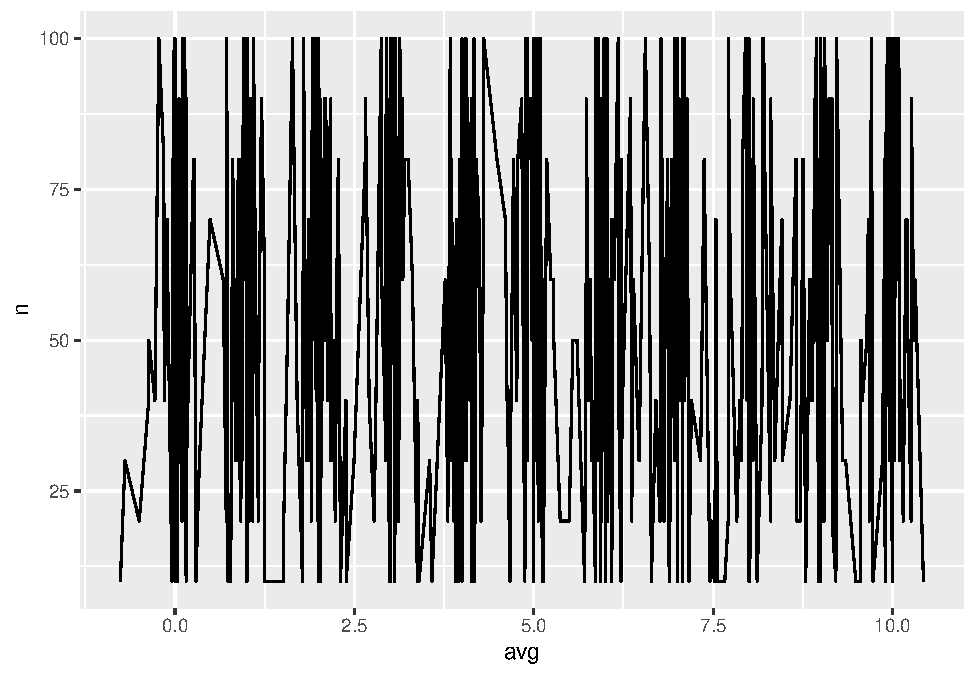
\includegraphics{Seminararbeit_files/figure-latex/ggplot2-1.pdf}

\begin{itemize}

\item
  Visualizing average by using \texttt{facet\_grid()}
\end{itemize}

\begin{Shaded}
\begin{Highlighting}[]
\FunctionTok{ggplot}\NormalTok{(test\_me}\SpecialCharTok{$}\NormalTok{average,}\FunctionTok{aes}\NormalTok{(}\AttributeTok{x=}\NormalTok{avg))}\SpecialCharTok{+}\FunctionTok{facet\_grid}\NormalTok{(n}\SpecialCharTok{\textasciitilde{}}\NormalTok{.)}\SpecialCharTok{+}
  \FunctionTok{geom\_density}\NormalTok{()}
\end{Highlighting}
\end{Shaded}

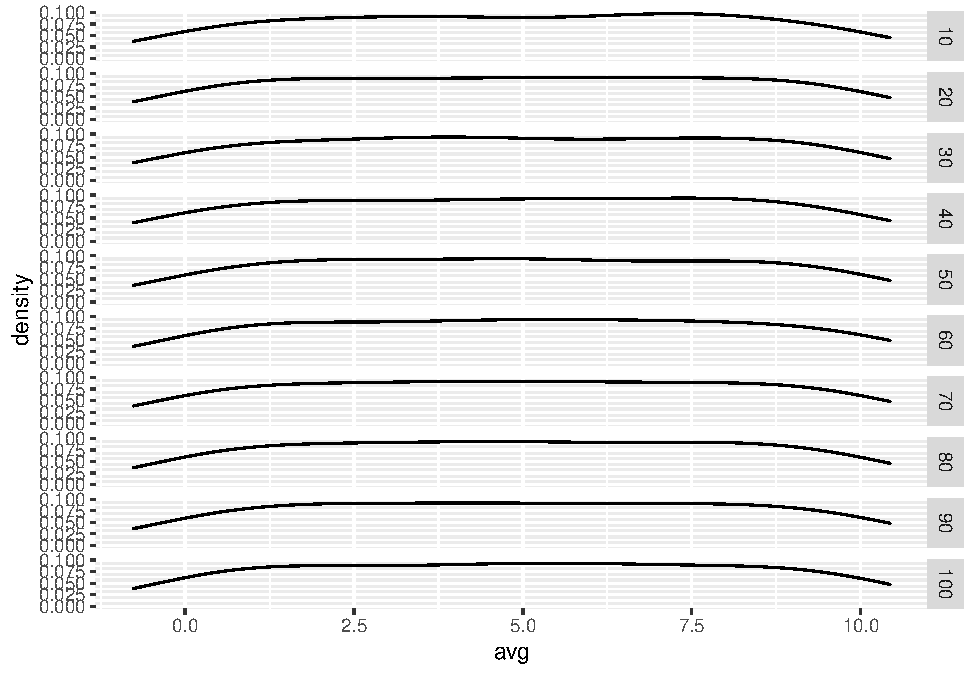
\includegraphics{Seminararbeit_files/figure-latex/facet-1.pdf} As given
graphs above, the simulation result works well with \texttt{ggplot2}
methods.

\hypertarget{examples}{%
\section{Examples}\label{examples}}

\hypertarget{comparing-the-execution-times-of-ols-and-gls-simulations}{%
\subsection{Comparing the execution times of OLS and GLS
simulations}\label{comparing-the-execution-times-of-ols-and-gls-simulations}}

As an example of Monte Carlo simulation, OLS and GLS coefficients
\(\beta\) are simulated with and without parallelisation to compare the
execution time.

\begin{Shaded}
\begin{Highlighting}[]
\NormalTok{ols\_f }\OtherTok{\textless{}{-}} \ControlFlowTok{function}\NormalTok{(n,mu,sd)\{}
\NormalTok{  e }\OtherTok{\textless{}{-}} \FunctionTok{rnorm}\NormalTok{(n,mu,sd)}
\NormalTok{  x }\OtherTok{\textless{}{-}} \FunctionTok{runif}\NormalTok{(n)}
\NormalTok{  y }\OtherTok{\textless{}{-}} \FloatTok{0.5}\SpecialCharTok{*}\NormalTok{x }\SpecialCharTok{+}\NormalTok{ e}
\NormalTok{  ols.hat }\OtherTok{\textless{}{-}} \FunctionTok{t}\NormalTok{(x) }\SpecialCharTok{\%*\%}\NormalTok{ y }\SpecialCharTok{/} \FunctionTok{t}\NormalTok{(x)}\SpecialCharTok{\%*\%}\NormalTok{x}
  \FunctionTok{return}\NormalTok{(}\StringTok{"ols"}\OtherTok{=}\NormalTok{ols.hat)\}}

\NormalTok{gls\_f }\OtherTok{\textless{}{-}} \ControlFlowTok{function}\NormalTok{(n,mu,sd)\{}
\NormalTok{  e }\OtherTok{\textless{}{-}} \FunctionTok{rnorm}\NormalTok{(n,mu,sd)}
\NormalTok{  x }\OtherTok{\textless{}{-}} \FunctionTok{runif}\NormalTok{(n)}
\NormalTok{  y }\OtherTok{\textless{}{-}} \FloatTok{0.5}\SpecialCharTok{*}\NormalTok{x }\SpecialCharTok{+}\NormalTok{ e}
\NormalTok{  v.inv }\OtherTok{\textless{}{-}} \FunctionTok{diag}\NormalTok{(}\DecValTok{1}\SpecialCharTok{/}\NormalTok{(}\DecValTok{1}\SpecialCharTok{:}\NormalTok{n))}
\NormalTok{  c }\OtherTok{\textless{}{-}} \FunctionTok{chol}\NormalTok{(v.inv)}
\NormalTok{  cy }\OtherTok{\textless{}{-}}\NormalTok{ c }\SpecialCharTok{\%*\%}\NormalTok{ y}
\NormalTok{  cx }\OtherTok{\textless{}{-}}\NormalTok{ c }\SpecialCharTok{\%*\%}\NormalTok{ x}
\NormalTok{  gls\_hat }\OtherTok{\textless{}{-}} \FunctionTok{t}\NormalTok{(cx) }\SpecialCharTok{\%*\%}\NormalTok{ cy }\SpecialCharTok{/} \FunctionTok{t}\NormalTok{(cx)}\SpecialCharTok{\%*\%}\NormalTok{cx}
  \FunctionTok{return}\NormalTok{(}\StringTok{"gls"}\OtherTok{=}\NormalTok{gls\_hat)}
  
\NormalTok{  param\_list }\OtherTok{\textless{}{-}} \FunctionTok{list}\NormalTok{(}\FunctionTok{c}\NormalTok{(}\StringTok{"n"}\NormalTok{,}\DecValTok{100}\NormalTok{,}\DecValTok{1000}\NormalTok{,}\DecValTok{100}\NormalTok{),}\FunctionTok{c}\NormalTok{(}\StringTok{"mu"}\NormalTok{,}\DecValTok{0}\NormalTok{,}\DecValTok{1}\NormalTok{,}\FloatTok{0.25}\NormalTok{),}\FunctionTok{c}\NormalTok{(}\StringTok{"sd"}\NormalTok{,}\DecValTok{1}\NormalTok{,}\DecValTok{2}\NormalTok{,.}\DecValTok{5}\NormalTok{))}
\NormalTok{\}}
\end{Highlighting}
\end{Shaded}

As shown above, simple OLS and GLS functions are defined to find
\(\beta\) coefficients. However, the execution time of the GLS would be
much longer than OLS since The Cholesky Decomposition \texttt{chol()} is
applied to the GLS function.

\textbf{OLS simulation without parallel processing:}

\begin{Shaded}
\begin{Highlighting}[]
\NormalTok{ param\_list }\OtherTok{\textless{}{-}} \FunctionTok{list}\NormalTok{(}\FunctionTok{c}\NormalTok{(}\StringTok{"n"}\NormalTok{,}\DecValTok{100}\NormalTok{,}\DecValTok{1000}\NormalTok{,}\DecValTok{100}\NormalTok{),}\FunctionTok{c}\NormalTok{(}\StringTok{"mu"}\NormalTok{,}\DecValTok{0}\NormalTok{,}\DecValTok{1}\NormalTok{,}\FloatTok{0.25}\NormalTok{),}\FunctionTok{c}\NormalTok{(}\StringTok{"sd"}\NormalTok{,}\DecValTok{1}\NormalTok{,}\DecValTok{2}\NormalTok{,.}\DecValTok{5}\NormalTok{))}
\NormalTok{ols }\OtherTok{\textless{}{-}} \FunctionTok{main\_function}\NormalTok{(}\AttributeTok{parameters =}\NormalTok{ param\_list,}
                     \AttributeTok{nrep=}\DecValTok{5}\NormalTok{,}
                     \AttributeTok{simulation =}\NormalTok{ ols\_f,}
                     \AttributeTok{sum\_fun=}\StringTok{"mean"}\NormalTok{,}
                     \AttributeTok{seed=}\DecValTok{123}\NormalTok{,}
                     \AttributeTok{cores=}\DecValTok{1}\NormalTok{)}
\end{Highlighting}
\end{Shaded}

\begin{verbatim}
## 
##  Repetition(nrep)      :  5 
## 
##  Parallelization Type  :  Sequential 
## 
##  Number of Cores Used in  Parallelization :  1  out of 8 
## 
##  Input Parameters :  c("n", "100", "1000", "100") c("mu", "0", "1", "0.25") c("sd", "1", "2", "0.5") 
## 
##  Simulation Length : 750 
##  Minumum : 0.08611764 
##  Maximum : 2.598461 
##  Mean    : 1.251827 
##  Median  : 1.246948 
## 
##  Execution Time of Monte Carlo Simulation 0.09394312 secs 
## 
##  Name of The Class : Eco
\end{verbatim}

The total execution time of OLS simulation is 8.46 seconds when only one
core is used.

\textbf{OLS simulation with parallel processing:}

\begin{Shaded}
\begin{Highlighting}[]
\NormalTok{ols }\OtherTok{\textless{}{-}} \FunctionTok{main\_function}\NormalTok{(}\AttributeTok{parameters =}\NormalTok{ param\_list,}
                     \AttributeTok{nrep=}\DecValTok{5}\NormalTok{,}
                     \AttributeTok{simulation =}\NormalTok{ ols\_f,}
                     \AttributeTok{sum\_fun=}\StringTok{"mean"}\NormalTok{,}
                     \AttributeTok{seed=}\DecValTok{123}\NormalTok{,}
                     \AttributeTok{cores=}\DecValTok{4}\NormalTok{)}
\end{Highlighting}
\end{Shaded}

\begin{verbatim}
## 
##  Repetition(nrep)      :  5 
## 
##  Parallelization Type  :  Multisession 
## 
##  Number of Cores Used in  Parallelization :  4  out of 8 
## 
##  Input Parameters :  c("n", "100", "1000", "100") c("mu", "0", "1", "0.25") c("sd", "1", "2", "0.5") 
## 
##  Simulation Length : 750 
##  Minumum : 0.08611764 
##  Maximum : 2.598461 
##  Mean    : 1.251827 
##  Median  : 1.246948 
## 
##  Execution Time of Monte Carlo Simulation 1.138782 secs 
## 
##  Name of The Class : Eco
\end{verbatim}

The total execution time of OLS simulation is 12 seconds when only four
core is used.

\textbf{GLS with parallel processing:}

\begin{Shaded}
\begin{Highlighting}[]
\NormalTok{gls }\OtherTok{\textless{}{-}} \FunctionTok{main\_function}\NormalTok{(}\AttributeTok{parameters =}\NormalTok{ param\_list,}
                     \AttributeTok{nrep=}\DecValTok{5}\NormalTok{,}
                     \AttributeTok{simulation =}\NormalTok{ gls\_f,}
                     \AttributeTok{sum\_fun=}\StringTok{"mean"}\NormalTok{,}
                     \AttributeTok{seed=}\DecValTok{123}\NormalTok{,}
                     \AttributeTok{cores=}\DecValTok{4}\NormalTok{)}
\end{Highlighting}
\end{Shaded}

\begin{verbatim}
## 
##  Repetition(nrep)      :  5 
## 
##  Parallelization Type  :  Multisession 
## 
##  Number of Cores Used in  Parallelization :  4  out of 8 
## 
##  Input Parameters :  c("n", "100", "1000", "100") c("mu", "0", "1", "0.25") c("sd", "1", "2", "0.5") 
## 
##  Simulation Length : 750 
##  Minumum : -0.9971 
##  Maximum : 3.383637 
##  Mean    : 1.260196 
##  Median  : 1.284057 
## 
##  Execution Time of Monte Carlo Simulation 29.96168 secs 
## 
##  Name of The Class : Eco
\end{verbatim}

\textbf{GLS without parallel processing:}

\begin{Shaded}
\begin{Highlighting}[]
\NormalTok{gls }\OtherTok{\textless{}{-}} \FunctionTok{main\_function}\NormalTok{(}\AttributeTok{parameters =}\NormalTok{ param\_list,}
                     \AttributeTok{nrep=}\DecValTok{5}\NormalTok{,}
                     \AttributeTok{simulation =}\NormalTok{ gls\_f,}
                     \AttributeTok{sum\_fun=}\StringTok{"mean"}\NormalTok{,}
                     \AttributeTok{seed=}\DecValTok{123}\NormalTok{,}
                     \AttributeTok{cores=}\DecValTok{1}\NormalTok{)}
\end{Highlighting}
\end{Shaded}

\begin{verbatim}
## 
##  Repetition(nrep)      :  5 
## 
##  Parallelization Type  :  Sequential 
## 
##  Number of Cores Used in  Parallelization :  1  out of 8 
## 
##  Input Parameters :  c("n", "100", "1000", "100") c("mu", "0", "1", "0.25") c("sd", "1", "2", "0.5") 
## 
##  Simulation Length : 750 
##  Minumum : -0.9971 
##  Maximum : 3.383637 
##  Mean    : 1.260196 
##  Median  : 1.284057 
## 
##  Execution Time of Monte Carlo Simulation 28.80312 secs 
## 
##  Name of The Class : Eco
\end{verbatim}

As seen in the summary part, the total execution time of the simulation
took 36.35 seconds which also proves that the parallel process works
well. Therefore, execution times of the simulation might differ on other
computers.

\hypertarget{visualisation}{%
\subsection{Visualisation}\label{visualisation}}

\textbf{Visualizing MSE(Mean Square Error) in OLS and GLS simulations:}

MSE is calculated by \texttt{out\$average\$mse} for each simulation.

\begin{Shaded}
\begin{Highlighting}[]
\NormalTok{gls}\SpecialCharTok{$}\NormalTok{average }\OtherTok{\textless{}{-}}\NormalTok{  gls}\SpecialCharTok{$}\NormalTok{average }\SpecialCharTok{\%\textgreater{}\%} \FunctionTok{mutate}\NormalTok{(}\AttributeTok{mse =}\NormalTok{(}\DecValTok{2}\SpecialCharTok{{-}}\NormalTok{avg)}\SpecialCharTok{\^{}}\DecValTok{2}\NormalTok{ )}
\NormalTok{ols}\SpecialCharTok{$}\NormalTok{average }\OtherTok{\textless{}{-}}\NormalTok{  ols}\SpecialCharTok{$}\NormalTok{average }\SpecialCharTok{\%\textgreater{}\%} \FunctionTok{mutate}\NormalTok{(}\AttributeTok{mse =}\NormalTok{(}\DecValTok{2}\SpecialCharTok{{-}}\NormalTok{avg)}\SpecialCharTok{\^{}}\DecValTok{2}\NormalTok{ )}

\NormalTok{ols}\SpecialCharTok{$}\NormalTok{average }\SpecialCharTok{\%\textgreater{}\%} \FunctionTok{ggplot}\NormalTok{(}\FunctionTok{aes}\NormalTok{(}\AttributeTok{x=}\NormalTok{avg,}\AttributeTok{y=}\NormalTok{mu,}\AttributeTok{col=}\StringTok{"OLS"}\NormalTok{))}\SpecialCharTok{+}
  \FunctionTok{facet\_grid}\NormalTok{(n}\SpecialCharTok{\textasciitilde{}}\FunctionTok{mean}\NormalTok{(mse))}\SpecialCharTok{+}\FunctionTok{geom\_line}\NormalTok{()}\SpecialCharTok{+}
 \FunctionTok{geom\_line}\NormalTok{(}\AttributeTok{data=}\NormalTok{gls}\SpecialCharTok{$}\NormalTok{average,}\FunctionTok{aes}\NormalTok{(}\AttributeTok{x=}\NormalTok{avg,}\AttributeTok{y=}\NormalTok{mu,}\AttributeTok{col=}\StringTok{"GLS"}\NormalTok{))}\SpecialCharTok{+}
  \FunctionTok{scale\_color\_manual}\NormalTok{(}\AttributeTok{name =} \StringTok{"Estimation"}\NormalTok{,}
                     \AttributeTok{values =} \FunctionTok{c}\NormalTok{(}\StringTok{"OLS"} \OtherTok{=} \StringTok{"blue"}\NormalTok{, }\StringTok{"GLS"} \OtherTok{=} \StringTok{"red"}\NormalTok{))}
\end{Highlighting}
\end{Shaded}

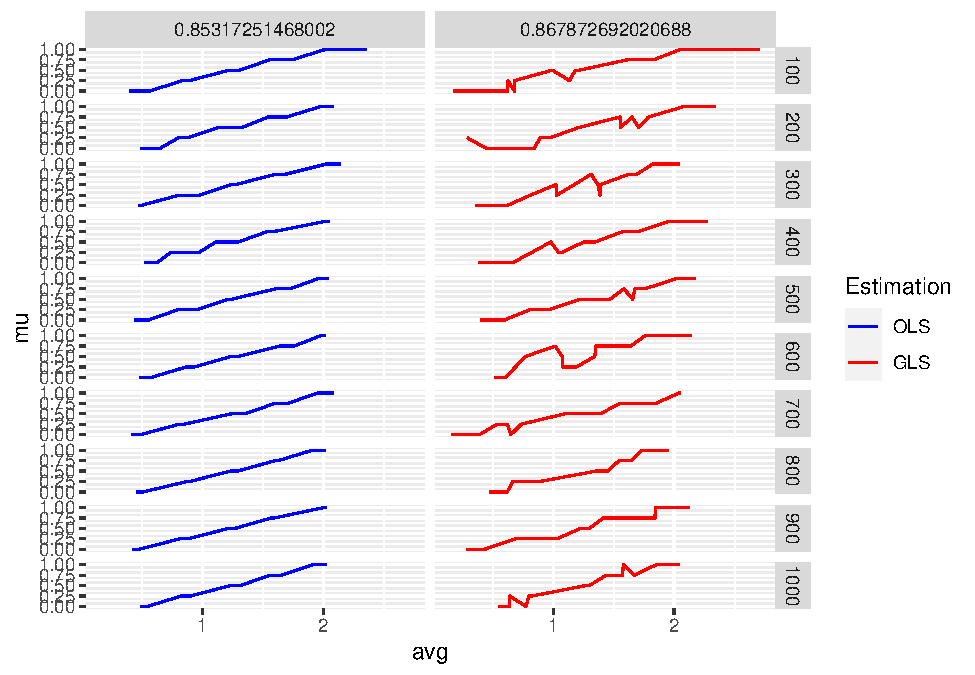
\includegraphics{Seminararbeit_files/figure-latex/unnamed-chunk-4-1.pdf}
\pagebreak

\textbf{Density graph of MSE of \(\beta\) in OLS and GLS simulations}

\begin{Shaded}
\begin{Highlighting}[]
\FunctionTok{ggplot}\NormalTok{(ols}\SpecialCharTok{$}\NormalTok{average,}\FunctionTok{aes}\NormalTok{(}\AttributeTok{x=}\NormalTok{mse,}\AttributeTok{col=}\StringTok{"OLS"}\NormalTok{))}\SpecialCharTok{+}\FunctionTok{facet\_grid}\NormalTok{(n}\SpecialCharTok{\textasciitilde{}}\NormalTok{.)}\SpecialCharTok{+}
  \FunctionTok{geom\_density}\NormalTok{()}\SpecialCharTok{+}
  \FunctionTok{geom\_density}\NormalTok{(}\AttributeTok{data=}\NormalTok{gls}\SpecialCharTok{$}\NormalTok{average,}\FunctionTok{aes}\NormalTok{(}\AttributeTok{x=}\NormalTok{avg,}\AttributeTok{col=}\StringTok{"GLS"}\NormalTok{))}\SpecialCharTok{+}
  \FunctionTok{scale\_color\_manual}\NormalTok{(}\AttributeTok{name =} \StringTok{"Estimation"}\NormalTok{, }
                     \AttributeTok{values =} \FunctionTok{c}\NormalTok{(}\StringTok{"OLS"} \OtherTok{=} \StringTok{"blue"}\NormalTok{, }\StringTok{"GLS"} \OtherTok{=} \StringTok{"red"}\NormalTok{))}
\end{Highlighting}
\end{Shaded}

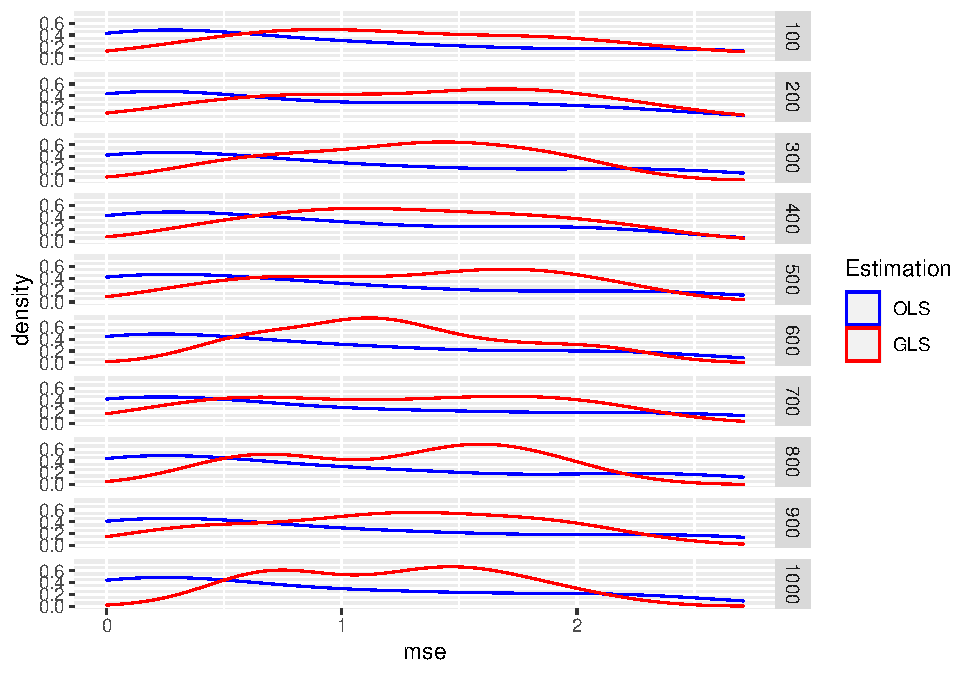
\includegraphics{Seminararbeit_files/figure-latex/unnamed-chunk-5-1.pdf}

\pagebreak

\hypertarget{conclusion}{%
\section{Conclusion}\label{conclusion}}

The above section illustrates the power of the implemented model and
provides the fairly easy-to-use tool that still allows for various
specifications in terms of used parameters, data generation processes
and summary functions. Researchers, who use Monte Carlo studies
regularly may save much time using a tool like this in the long run.

By nature, there may be cases, where the implementation does not satisfy
the user's needs to the fullest, but for a wide variety of examples it
is showed, it worked well and served the over all purpose. Furthermore,
the functional programming approach allows for easy and flexible
adjustments in case the use of the functions should be expanded, such as
if a grid of more than 3 (or 4?) parameters is
needed.???????????????????????????????????????????????????

\pagebreak

\hypertarget{contributions}{%
\section{Contributions}\label{contributions}}

\begin{longtable}[]{@{}cccc@{}}
\toprule()
& Alexander Langnau & Öcal Kaptan & Sunyoung Ji \\
\midrule()
\endhead
Planning & 0 & 0 & 0 \\
Create\_grid & 0 & 0 & 0 \\
Data\_generation & 0 & 0 & 0 \\
Summary\_function & 0 & 0 & 0 \\
Create\_array\_function & 0 & 0 & 0 \\
Average\_function & 0 & 0 & 0 \\
Output\_function & 0 & 0 & 0 \\
ggplot2 part & 0 & 0 & 0 \\
Parallelisation & 0 & 0 & 0 \\
Formatting & 0 & 0 & 0 \\
Writing the report & 0 & 0 & 0 \\
Proof-reading & 0 & 0 & 0 \\
\bottomrule()
\end{longtable}

\pagebreak

\hypertarget{references}{%
\section{References}\label{references}}

Adrian G. Barbu, Song Chun Zhu, ``Monte Carlo Methods'', Springer
Singapore, 2020, pp.1-4,
\url{doi:https://doi.org/10.1007/978-981-13-2971-5}\\

Czech, Z. ``In Introduction to Parallel Computing'', Cambridge
University Press, 2017, pp.~1-34, \url{doi:10.1017/9781316795835.002}

rdocumentation.org, DataCamp, ``cat: Concatenate and Print'',
url:\url{https://www.rdocumentation.org/packages/base/versions/3.6.2/topics/cat}

\pagebreak

\hypertarget{appendix}{%
\section{Appendix}\label{appendix}}

\hypertarget{appendix-a}{%
\subsection{Appendix A}\label{appendix-a}}

\textbf{Output of the OLS simulation}

\begin{verbatim}
## 
##  Repetition(nrep)      :  5 
## 
##  Parallelization Type  :  Sequential 
## 
##  Number of Cores Used in  Parallelization :  1  out of 8 
## 
##  Input Parameters :  c("n", "100", "1000", "100") c("mu", "0", "1", "0.25") c("sd", "1", "2", "0.5") 
## 
##  Simulation Length : 750 
##  Minumum : 0.08611764 
##  Maximum : 2.598461 
##  Mean    : 1.251827 
##  Median  : 1.246948 
## 
##  Execution Time of Monte Carlo Simulation 0.08364701 secs 
## 
##  Name of The Class : Eco
\end{verbatim}

\begin{verbatim}
## $results
## , , sd=1, rep=1
## 
##             mu=0   mu=0.25   mu=0.5  mu=0.75     mu=1
## n=100  0.6824267 0.7726517 1.390428 1.352546 2.033425
## n=200  0.4786798 0.7268500 1.551036 1.469126 2.016927
## n=300  0.5430408 0.6925565 1.412873 1.516396 2.020209
## n=400  0.4916201 0.9335676 1.240309 1.588818 1.939011
## n=500  0.4665197 0.8658038 1.302298 1.621465 2.071480
## n=600  0.4135505 1.0087766 1.263624 1.564343 1.873183
## n=700  0.6062303 0.8060657 1.423163 1.677571 1.915217
## n=800  0.5215150 0.8373901 1.384251 1.536015 1.845518
## n=900  0.4377088 0.8522425 1.323030 1.625229 2.113246
## n=1000 0.4272311 0.9598533 1.171133 1.607383 2.007037
## 
## , , sd=1.5, rep=1
## 
##             mu=0   mu=0.25   mu=0.5  mu=0.75     mu=1
## n=100  0.2325414 0.8709612 1.007916 1.187153 1.646406
## n=200  0.2684302 0.5956376 1.066756 1.572480 1.780621
## n=300  0.3463280 0.5074475 1.249930 1.526170 2.281022
## n=400  0.5532419 0.6727324 1.069168 1.587438 2.040513
## n=500  0.5088940 0.9917867 1.254739 1.687302 2.191762
## n=600  0.5817868 1.0516531 1.388582 1.787617 2.039833
## n=700  0.4085830 0.9266206 1.177307 1.618533 1.795094
## n=800  0.4788177 0.7297284 1.261184 1.635941 1.990439
## n=900  0.4293894 0.7521720 1.281461 1.550926 1.969204
## n=1000 0.4379182 0.7061176 1.281116 1.604609 1.875328
## 
## , , sd=2, rep=1
## 
##             mu=0   mu=0.25   mu=0.5  mu=0.75     mu=1
## n=100  0.6237415 0.8008305 1.639701 1.897970 2.513486
## n=200  0.6110261 1.2155626 1.815507 1.725145 2.033192
## n=300  0.4066040 0.8631502 1.239882 1.684178 2.106188
## n=400  0.4235146 0.6718906 1.072217 1.373997 2.000179
## n=500  0.4979046 1.0646659 1.248795 1.624880 2.036934
## n=600  0.4167380 0.9594940 1.222973 1.538267 1.972503
## n=700  0.4474413 0.7043636 1.318657 1.298269 2.086695
## n=800  0.3558261 0.9032952 1.340988 1.480559 1.852471
## n=900  0.4184591 0.8440885 1.312351 1.481778 1.959888
## n=1000 0.5482327 0.8486597 1.325121 1.557654 2.174067
## 
## , , sd=1, rep=2
## 
##             mu=0   mu=0.25   mu=0.5  mu=0.75     mu=1
## n=100  0.5699594 0.6347600 1.240574 1.409578 2.102247
## n=200  0.3411974 0.9859774 1.127496 1.654986 2.005527
## n=300  0.5568138 0.7710960 1.309760 1.640136 1.868297
## n=400  0.5892899 0.8630584 1.420656 1.488524 2.106760
## n=500  0.4565660 0.9875469 1.169863 1.642037 2.125870
## n=600  0.6074920 0.8311391 1.144387 1.561809 2.127146
## n=700  0.5311162 0.8793250 1.213227 1.758464 2.019087
## n=800  0.4907978 0.8137087 1.243065 1.544169 1.890569
## n=900  0.5006696 0.9126527 1.185916 1.551420 2.011440
## n=1000 0.5132049 0.8425093 1.323331 1.665086 2.067430
## 
## , , sd=1.5, rep=2
## 
##             mu=0   mu=0.25    mu=0.5  mu=0.75     mu=1
## n=100  0.4100172 1.0050342 1.3586338 1.594119 2.030257
## n=200  0.7621120 1.1129076 1.2050693 1.766159 2.052134
## n=300  0.4495498 0.9131922 1.3998834 1.844595 2.048539
## n=400  0.5189146 0.9392205 0.9085613 1.502305 2.159537
## n=500  0.7089984 0.6966299 1.1168839 1.472302 1.942223
## n=600  0.3991638 0.7265354 1.1572410 1.748560 1.735354
## n=700  0.4141086 0.7800295 1.3853238 1.765437 1.860513
## n=800  0.3797112 0.8637205 1.1967238 1.669677 1.904555
## n=900  0.4946693 0.9968749 1.3024325 1.747231 2.093768
## n=1000 0.6315810 0.8282354 1.1035843 1.541674 1.946093
## 
## , , sd=2, rep=2
## 
##             mu=0   mu=0.25    mu=0.5  mu=0.75     mu=1
## n=100  0.2670268 1.0417428 0.9765324 1.779177 2.139938
## n=200  0.2064741 0.8966665 1.2011619 1.562213 1.929578
## n=300  0.2953656 0.8280923 1.4380720 1.301385 2.089569
## n=400  0.7044943 0.8050854 1.4651276 1.320472 2.051137
## n=500  0.4125427 0.8432624 0.9844522 1.838044 2.144216
## n=600  0.7200719 0.9085732 1.0035755 1.809966 2.205790
## n=700  0.5352158 0.8738860 1.2227186 1.564884 2.114450
## n=800  0.3849922 0.7982686 1.2963208 1.625716 1.980291
## n=900  0.3505717 0.7606954 1.0653161 1.494651 1.986403
## n=1000 0.5160520 0.8734081 1.3842792 1.766722 2.085573
## 
## , , sd=1, rep=3
## 
##             mu=0   mu=0.25   mu=0.5  mu=0.75     mu=1
## n=100  0.5968253 1.0425781 1.207359 1.494982 1.755818
## n=200  0.6013728 0.8169956 1.089477 1.759701 2.050444
## n=300  0.4185383 0.8722548 1.202220 1.632546 2.054984
## n=400  0.5761413 0.9439121 1.215469 1.611440 2.019500
## n=500  0.6625234 0.8265606 1.301594 1.551010 1.973081
## n=600  0.6338517 0.9970815 1.257844 1.716586 2.047527
## n=700  0.4954136 0.8538731 1.202218 1.656197 1.921142
## n=800  0.4847987 0.8606272 1.280399 1.681161 1.939804
## n=900  0.4581839 0.8963640 1.363804 1.640401 2.005699
## n=1000 0.4964781 0.9341992 1.243164 1.696117 1.985360
## 
## , , sd=1.5, rep=3
## 
##             mu=0   mu=0.25   mu=0.5  mu=0.75     mu=1
## n=100  0.5659700 0.7903221 1.254210 1.886166 1.790293
## n=200  0.5821258 0.6511703 1.343681 1.782181 1.894019
## n=300  0.6550444 0.9367739 1.380756 1.705998 2.028275
## n=400  0.7048194 0.9633662 1.120887 1.688024 1.811344
## n=500  0.3923555 0.7626086 1.104116 1.537444 2.047353
## n=600  0.4717144 0.8688271 1.175261 1.826726 1.983990
## n=700  0.3871651 0.6201482 1.305263 1.669981 2.042779
## n=800  0.4834246 0.9357010 1.305622 1.523736 2.081715
## n=900  0.4433156 0.7916531 1.359010 1.580634 1.940405
## n=1000 0.4946876 0.8067392 1.480151 1.486763 1.900808
## 
## , , sd=2, rep=3
## 
##             mu=0   mu=0.25    mu=0.5  mu=0.75     mu=1
## n=100  0.4237920 0.5144245 0.4718755 2.004104 2.186295
## n=200  0.5777614 0.7299343 1.6298909 1.499530 1.929751
## n=300  0.6276662 0.8600749 0.9626478 2.011661 2.175176
## n=400  0.5785860 0.9158230 1.1544399 1.389809 2.169336
## n=500  0.2516702 0.9907678 1.0602298 1.532465 1.682624
## n=600  0.5165529 0.8616768 1.5189127 1.652623 1.941119
## n=700  0.4674128 0.7479103 1.2133761 1.738886 1.996975
## n=800  0.5090721 0.8062749 1.3959268 1.542798 1.994769
## n=900  0.4197560 0.8280591 1.2129929 1.504396 1.947569
## n=1000 0.6527630 0.8873246 1.2662086 1.656169 2.115128
## 
## , , sd=1, rep=4
## 
##             mu=0   mu=0.25    mu=0.5  mu=0.75     mu=1
## n=100  0.7359835 1.0087000 1.1157127 1.851686 2.286974
## n=200  0.5466285 0.8691083 0.9809655 1.677466 1.914859
## n=300  0.4092951 0.8421824 1.1834134 1.463671 2.105769
## n=400  0.4870693 0.8787365 1.3442915 1.641625 2.038680
## n=500  0.6247941 0.9737552 1.1814126 1.583607 1.981457
## n=600  0.5543342 0.9385104 1.2433161 1.676785 1.916412
## n=700  0.4178732 0.8808745 1.1952781 1.530920 1.960542
## n=800  0.5618498 0.8943310 1.2475019 1.686068 1.946561
## n=900  0.5052058 0.8785736 1.2679218 1.571624 2.009535
## n=1000 0.4550461 0.8622264 1.2189931 1.640547 2.027112
## 
## , , sd=1.5, rep=4
## 
##             mu=0   mu=0.25    mu=0.5  mu=0.75     mu=1
## n=100  0.4449720 0.8435500 1.5231357 1.528876 2.461235
## n=200  0.3352203 0.8038153 0.9593336 1.823112 2.149320
## n=300  0.4930487 0.6791231 1.0272955 1.574880 2.304307
## n=400  0.3806721 1.1714969 1.4056411 1.543264 2.258722
## n=500  0.4589277 0.7928819 1.5044037 1.632672 1.829121
## n=600  0.4884702 0.6958911 1.2883971 1.606977 2.109358
## n=700  0.5038252 0.8396545 1.4939591 1.598702 2.198315
## n=800  0.5515391 0.8256058 1.2838778 1.644795 2.020077
## n=900  0.4102779 0.7769137 1.2511958 1.567744 1.925168
## n=1000 0.6885496 0.9734467 1.2688095 1.525439 1.946295
## 
## , , sd=2, rep=4
## 
##             mu=0   mu=0.25    mu=0.5  mu=0.75     mu=1
## n=100  0.5717011 0.8796835 2.1004676 1.351107 2.598461
## n=200  1.1810891 0.4725781 0.9070217 1.490537 2.444452
## n=300  0.5900949 1.0569764 1.3134750 1.766744 2.089249
## n=400  0.7380901 0.4503391 1.0841655 1.704982 1.998472
## n=500  0.6158445 1.0384364 1.6255235 1.911106 1.868147
## n=600  0.6300586 1.1140343 1.1895053 1.822727 1.933571
## n=700  0.3625215 0.9113498 1.2522415 1.654996 1.981563
## n=800  0.4427674 0.8570775 1.1367413 1.796147 2.103874
## n=900  0.3816606 0.8423425 1.3168243 1.712630 2.102760
## n=1000 0.4265370 0.9495205 1.3021528 1.603875 1.875588
## 
## , , sd=1, rep=5
## 
##             mu=0   mu=0.25   mu=0.5  mu=0.75     mu=1
## n=100  0.2288956 0.9259850 1.345124 1.767008 1.904891
## n=200  0.4782098 0.9611524 1.326272 1.689215 2.050280
## n=300  0.4520819 0.9920557 1.238380 1.753581 2.087970
## n=400  0.4573970 1.1576259 1.246390 1.497974 2.019858
## n=500  0.5434649 0.9485599 1.191573 1.631702 2.049623
## n=600  0.4632066 0.8962950 1.266618 1.657375 1.924914
## n=700  0.3907963 0.8164093 1.155234 1.615976 1.949318
## n=800  0.4930138 0.9572131 1.295102 1.684709 1.936302
## n=900  0.4979275 0.8736681 1.214887 1.584737 1.985072
## n=1000 0.5301261 0.8977935 1.313722 1.630559 1.935747
## 
## , , sd=1.5, rep=5
## 
##             mu=0   mu=0.25   mu=0.5  mu=0.75     mu=1
## n=100  0.4688968 0.9435859 1.380401 1.586464 2.192555
## n=200  0.7831954 0.8507725 1.104056 1.524999 1.987862
## n=300  0.4957244 0.9953593 1.100958 1.596888 2.032147
## n=400  0.6377009 1.1108968 1.039524 1.621890 1.989716
## n=500  0.2757090 0.7425858 1.221020 1.687816 1.782811
## n=600  0.4674703 0.9888671 1.462157 1.805296 2.070940
## n=700  0.3602414 0.8718152 1.369915 1.868538 1.981321
## n=800  0.3886475 1.1178513 1.246394 1.612441 2.065348
## n=900  0.4814983 0.8016443 1.148795 1.443979 2.099358
## n=1000 0.4683020 0.8041379 1.013566 1.662726 1.873865
## 
## , , sd=2, rep=5
## 
##              mu=0   mu=0.25    mu=0.5  mu=0.75     mu=1
## n=100  0.08611764 0.9398614 0.9146867 1.669708 2.319204
## n=200  0.67138321 0.6832920 1.0754579 1.433456 2.068870
## n=300  0.44312742 1.2584762 1.3301563 1.650963 2.100398
## n=400  0.66455181 0.8364694 1.2167647 1.894041 1.989744
## n=500  0.41708387 0.8419375 1.1330271 1.713047 2.102631
## n=600  0.60004510 0.7267214 1.2282300 1.533603 2.044685
## n=700  0.42035536 0.8611750 1.3460957 1.744825 2.228779
## n=800  0.59792089 1.0213057 0.9896550 1.553520 1.600474
## n=900  0.51242473 0.7970967 1.1751429 1.646252 2.039864
## n=1000 0.56705287 0.8053208 1.2585926 1.673913 1.889833
## 
## attr(,"class")
## [1] "Eco"   "array"
## 
## $average
##        n   mu  sd       avg
## 1    100 0.00 1.0 0.5628181
## 2    100 0.00 1.5 0.4244795
## 3    100 0.00 2.0 0.3944758
## 4    100 0.25 1.0 0.8769350
## 5    100 0.25 1.5 0.8906907
## 6    100 0.25 2.0 0.8353085
## 7    100 0.50 1.0 1.2598397
## 8    100 0.50 1.5 1.3048593
## 9    100 0.50 2.0 1.2206527
## 10   100 0.75 1.0 1.5751601
## 11   100 0.75 1.5 1.5565558
## 12   100 0.75 2.0 1.7404132
## 13   100 1.00 1.0 2.0166709
## 14   100 1.00 1.5 2.0241493
## 15   100 1.00 2.0 2.3514768
## 16   200 0.00 1.0 0.4892177
## 17   200 0.00 1.5 0.5462168
## 18   200 0.00 2.0 0.6495468
## 19   200 0.25 1.0 0.8720167
## 20   200 0.25 1.5 0.8028606
## 21   200 0.25 2.0 0.7996067
## 22   200 0.50 1.0 1.2150492
## 23   200 0.50 1.5 1.1357791
## 24   200 0.50 2.0 1.3258080
## 25   200 0.75 1.0 1.6500989
## 26   200 0.75 1.5 1.6937863
## 27   200 0.75 2.0 1.5421762
## 28   200 1.00 1.0 2.0076074
## 29   200 1.00 1.5 1.9727911
## 30   200 1.00 2.0 2.0811684
## 31   300 0.00 1.0 0.4759540
## 32   300 0.00 1.5 0.4879391
## 33   300 0.00 2.0 0.4725716
## 34   300 0.25 1.0 0.8340291
## 35   300 0.25 1.5 0.8063792
## 36   300 0.25 2.0 0.9733540
## 37   300 0.50 1.0 1.2693292
## 38   300 0.50 1.5 1.2317647
## 39   300 0.50 2.0 1.2568465
## 40   300 0.75 1.0 1.6012659
## 41   300 0.75 1.5 1.6497061
## 42   300 0.75 2.0 1.6829863
## 43   300 1.00 1.0 2.0274458
## 44   300 1.00 1.5 2.1388580
## 45   300 1.00 2.0 2.1121160
## 46   400 0.00 1.0 0.5203035
## 47   400 0.00 1.5 0.5590698
## 48   400 0.00 2.0 0.6218474
## 49   400 0.25 1.0 0.9553801
## 50   400 0.25 1.5 0.9715426
## 51   400 0.25 2.0 0.7359215
## 52   400 0.50 1.0 1.2934233
## 53   400 0.50 1.5 1.1087563
## 54   400 0.50 2.0 1.1985429
## 55   400 0.75 1.0 1.5656764
## 56   400 0.75 1.5 1.5885842
## 57   400 0.75 2.0 1.5366603
## 58   400 1.00 1.0 2.0247618
## 59   400 1.00 1.5 2.0519664
## 60   400 1.00 2.0 2.0417733
## 61   500 0.00 1.0 0.5507736
## 62   500 0.00 1.5 0.4689769
## 63   500 0.00 2.0 0.4390092
## 64   500 0.25 1.0 0.9204453
## 65   500 0.25 1.5 0.7972986
## 66   500 0.25 2.0 0.9558140
## 67   500 0.50 1.0 1.2293479
## 68   500 0.50 1.5 1.2402327
## 69   500 0.50 2.0 1.2104054
## 70   500 0.75 1.0 1.6059639
## 71   500 0.75 1.5 1.6035074
## 72   500 0.75 2.0 1.7239084
## 73   500 1.00 1.0 2.0403021
## 74   500 1.00 1.5 1.9586539
## 75   500 1.00 2.0 1.9669104
## 76   600 0.00 1.0 0.5344870
## 77   600 0.00 1.5 0.4817211
## 78   600 0.00 2.0 0.5766933
## 79   600 0.25 1.0 0.9343605
## 80   600 0.25 1.5 0.8663548
## 81   600 0.25 2.0 0.9141000
## 82   600 0.50 1.0 1.2351578
## 83   600 0.50 1.5 1.2943275
## 84   600 0.50 2.0 1.2326393
## 85   600 0.75 1.0 1.6353797
## 86   600 0.75 1.5 1.7550350
## 87   600 0.75 2.0 1.6714372
## 88   600 1.00 1.0 1.9778364
## 89   600 1.00 1.5 1.9878951
## 90   600 1.00 2.0 2.0195340
## 91   700 0.00 1.0 0.4882859
## 92   700 0.00 1.5 0.4147847
## 93   700 0.00 2.0 0.4465893
## 94   700 0.25 1.0 0.8473095
## 95   700 0.25 1.5 0.8076536
## 96   700 0.25 2.0 0.8197369
## 97   700 0.50 1.0 1.2378238
## 98   700 0.50 1.5 1.3463535
## 99   700 0.50 2.0 1.2706179
## 100  700 0.75 1.0 1.6478257
## 101  700 0.75 1.5 1.7042384
## 102  700 0.75 2.0 1.6003720
## 103  700 1.00 1.0 1.9530612
## 104  700 1.00 1.5 1.9756043
## 105  700 1.00 2.0 2.0816926
## 106  800 0.00 1.0 0.5103950
## 107  800 0.00 1.5 0.4564280
## 108  800 0.00 2.0 0.4581157
## 109  800 0.25 1.0 0.8726540
## 110  800 0.25 1.5 0.8945214
## 111  800 0.25 2.0 0.8772444
## 112  800 0.50 1.0 1.2900639
## 113  800 0.50 1.5 1.2587603
## 114  800 0.50 2.0 1.2319263
## 115  800 0.75 1.0 1.6264243
## 116  800 0.75 1.5 1.6173179
## 117  800 0.75 2.0 1.5997479
## 118  800 1.00 1.0 1.9117509
## 119  800 1.00 1.5 2.0124269
## 120  800 1.00 2.0 1.9063757
## 121  900 0.00 1.0 0.4799391
## 122  900 0.00 1.5 0.4518301
## 123  900 0.00 2.0 0.4165744
## 124  900 0.25 1.0 0.8827002
## 125  900 0.25 1.5 0.8238516
## 126  900 0.25 2.0 0.8144564
## 127  900 0.50 1.0 1.2711118
## 128  900 0.50 1.5 1.2685788
## 129  900 0.50 2.0 1.2165253
## 130  900 0.75 1.0 1.5946823
## 131  900 0.75 1.5 1.5781026
## 132  900 0.75 2.0 1.5679413
## 133  900 1.00 1.0 2.0249983
## 134  900 1.00 1.5 2.0055806
## 135  900 1.00 2.0 2.0072967
## 136 1000 0.00 1.0 0.4844173
## 137 1000 0.00 1.5 0.5442077
## 138 1000 0.00 2.0 0.5421275
## 139 1000 0.25 1.0 0.8993163
## 140 1000 0.25 1.5 0.8237354
## 141 1000 0.25 2.0 0.8728468
## 142 1000 0.50 1.0 1.2540685
## 143 1000 0.50 1.5 1.2294453
## 144 1000 0.50 2.0 1.3072707
## 145 1000 0.75 1.0 1.6479383
## 146 1000 0.75 1.5 1.5642421
## 147 1000 0.75 2.0 1.6516665
## 148 1000 1.00 1.0 2.0045373
## 149 1000 1.00 1.5 1.9084779
## 150 1000 1.00 2.0 2.0280377
## 
## attr(,"class")
## [1] "Eco"
\end{verbatim}

\pagebreak

\textbf{Output of the OLS simulation with parallelisation}

\begin{verbatim}
## 
##  Repetition(nrep)      :  5 
## 
##  Parallelization Type  :  Multisession 
## 
##  Number of Cores Used in  Parallelization :  4  out of 8 
## 
##  Input Parameters :  c("n", "100", "1000", "100") c("mu", "0", "1", "0.25") c("sd", "1", "2", "0.5") 
## 
##  Simulation Length : 750 
##  Minumum : 0.08611764 
##  Maximum : 2.598461 
##  Mean    : 1.251827 
##  Median  : 1.246948 
## 
##  Execution Time of Monte Carlo Simulation 0.716254 secs 
## 
##  Name of The Class : Eco
\end{verbatim}

\begin{verbatim}
## $results
## , , sd=1, rep=1
## 
##             mu=0   mu=0.25   mu=0.5  mu=0.75     mu=1
## n=100  0.6824267 0.7726517 1.390428 1.352546 2.033425
## n=200  0.4786798 0.7268500 1.551036 1.469126 2.016927
## n=300  0.5430408 0.6925565 1.412873 1.516396 2.020209
## n=400  0.4916201 0.9335676 1.240309 1.588818 1.939011
## n=500  0.4665197 0.8658038 1.302298 1.621465 2.071480
## n=600  0.4135505 1.0087766 1.263624 1.564343 1.873183
## n=700  0.6062303 0.8060657 1.423163 1.677571 1.915217
## n=800  0.5215150 0.8373901 1.384251 1.536015 1.845518
## n=900  0.4377088 0.8522425 1.323030 1.625229 2.113246
## n=1000 0.4272311 0.9598533 1.171133 1.607383 2.007037
## 
## , , sd=1.5, rep=1
## 
##             mu=0   mu=0.25   mu=0.5  mu=0.75     mu=1
## n=100  0.2325414 0.8709612 1.007916 1.187153 1.646406
## n=200  0.2684302 0.5956376 1.066756 1.572480 1.780621
## n=300  0.3463280 0.5074475 1.249930 1.526170 2.281022
## n=400  0.5532419 0.6727324 1.069168 1.587438 2.040513
## n=500  0.5088940 0.9917867 1.254739 1.687302 2.191762
## n=600  0.5817868 1.0516531 1.388582 1.787617 2.039833
## n=700  0.4085830 0.9266206 1.177307 1.618533 1.795094
## n=800  0.4788177 0.7297284 1.261184 1.635941 1.990439
## n=900  0.4293894 0.7521720 1.281461 1.550926 1.969204
## n=1000 0.4379182 0.7061176 1.281116 1.604609 1.875328
## 
## , , sd=2, rep=1
## 
##             mu=0   mu=0.25   mu=0.5  mu=0.75     mu=1
## n=100  0.6237415 0.8008305 1.639701 1.897970 2.513486
## n=200  0.6110261 1.2155626 1.815507 1.725145 2.033192
## n=300  0.4066040 0.8631502 1.239882 1.684178 2.106188
## n=400  0.4235146 0.6718906 1.072217 1.373997 2.000179
## n=500  0.4979046 1.0646659 1.248795 1.624880 2.036934
## n=600  0.4167380 0.9594940 1.222973 1.538267 1.972503
## n=700  0.4474413 0.7043636 1.318657 1.298269 2.086695
## n=800  0.3558261 0.9032952 1.340988 1.480559 1.852471
## n=900  0.4184591 0.8440885 1.312351 1.481778 1.959888
## n=1000 0.5482327 0.8486597 1.325121 1.557654 2.174067
## 
## , , sd=1, rep=2
## 
##             mu=0   mu=0.25   mu=0.5  mu=0.75     mu=1
## n=100  0.5699594 0.6347600 1.240574 1.409578 2.102247
## n=200  0.3411974 0.9859774 1.127496 1.654986 2.005527
## n=300  0.5568138 0.7710960 1.309760 1.640136 1.868297
## n=400  0.5892899 0.8630584 1.420656 1.488524 2.106760
## n=500  0.4565660 0.9875469 1.169863 1.642037 2.125870
## n=600  0.6074920 0.8311391 1.144387 1.561809 2.127146
## n=700  0.5311162 0.8793250 1.213227 1.758464 2.019087
## n=800  0.4907978 0.8137087 1.243065 1.544169 1.890569
## n=900  0.5006696 0.9126527 1.185916 1.551420 2.011440
## n=1000 0.5132049 0.8425093 1.323331 1.665086 2.067430
## 
## , , sd=1.5, rep=2
## 
##             mu=0   mu=0.25    mu=0.5  mu=0.75     mu=1
## n=100  0.4100172 1.0050342 1.3586338 1.594119 2.030257
## n=200  0.7621120 1.1129076 1.2050693 1.766159 2.052134
## n=300  0.4495498 0.9131922 1.3998834 1.844595 2.048539
## n=400  0.5189146 0.9392205 0.9085613 1.502305 2.159537
## n=500  0.7089984 0.6966299 1.1168839 1.472302 1.942223
## n=600  0.3991638 0.7265354 1.1572410 1.748560 1.735354
## n=700  0.4141086 0.7800295 1.3853238 1.765437 1.860513
## n=800  0.3797112 0.8637205 1.1967238 1.669677 1.904555
## n=900  0.4946693 0.9968749 1.3024325 1.747231 2.093768
## n=1000 0.6315810 0.8282354 1.1035843 1.541674 1.946093
## 
## , , sd=2, rep=2
## 
##             mu=0   mu=0.25    mu=0.5  mu=0.75     mu=1
## n=100  0.2670268 1.0417428 0.9765324 1.779177 2.139938
## n=200  0.2064741 0.8966665 1.2011619 1.562213 1.929578
## n=300  0.2953656 0.8280923 1.4380720 1.301385 2.089569
## n=400  0.7044943 0.8050854 1.4651276 1.320472 2.051137
## n=500  0.4125427 0.8432624 0.9844522 1.838044 2.144216
## n=600  0.7200719 0.9085732 1.0035755 1.809966 2.205790
## n=700  0.5352158 0.8738860 1.2227186 1.564884 2.114450
## n=800  0.3849922 0.7982686 1.2963208 1.625716 1.980291
## n=900  0.3505717 0.7606954 1.0653161 1.494651 1.986403
## n=1000 0.5160520 0.8734081 1.3842792 1.766722 2.085573
## 
## , , sd=1, rep=3
## 
##             mu=0   mu=0.25   mu=0.5  mu=0.75     mu=1
## n=100  0.5968253 1.0425781 1.207359 1.494982 1.755818
## n=200  0.6013728 0.8169956 1.089477 1.759701 2.050444
## n=300  0.4185383 0.8722548 1.202220 1.632546 2.054984
## n=400  0.5761413 0.9439121 1.215469 1.611440 2.019500
## n=500  0.6625234 0.8265606 1.301594 1.551010 1.973081
## n=600  0.6338517 0.9970815 1.257844 1.716586 2.047527
## n=700  0.4954136 0.8538731 1.202218 1.656197 1.921142
## n=800  0.4847987 0.8606272 1.280399 1.681161 1.939804
## n=900  0.4581839 0.8963640 1.363804 1.640401 2.005699
## n=1000 0.4964781 0.9341992 1.243164 1.696117 1.985360
## 
## , , sd=1.5, rep=3
## 
##             mu=0   mu=0.25   mu=0.5  mu=0.75     mu=1
## n=100  0.5659700 0.7903221 1.254210 1.886166 1.790293
## n=200  0.5821258 0.6511703 1.343681 1.782181 1.894019
## n=300  0.6550444 0.9367739 1.380756 1.705998 2.028275
## n=400  0.7048194 0.9633662 1.120887 1.688024 1.811344
## n=500  0.3923555 0.7626086 1.104116 1.537444 2.047353
## n=600  0.4717144 0.8688271 1.175261 1.826726 1.983990
## n=700  0.3871651 0.6201482 1.305263 1.669981 2.042779
## n=800  0.4834246 0.9357010 1.305622 1.523736 2.081715
## n=900  0.4433156 0.7916531 1.359010 1.580634 1.940405
## n=1000 0.4946876 0.8067392 1.480151 1.486763 1.900808
## 
## , , sd=2, rep=3
## 
##             mu=0   mu=0.25    mu=0.5  mu=0.75     mu=1
## n=100  0.4237920 0.5144245 0.4718755 2.004104 2.186295
## n=200  0.5777614 0.7299343 1.6298909 1.499530 1.929751
## n=300  0.6276662 0.8600749 0.9626478 2.011661 2.175176
## n=400  0.5785860 0.9158230 1.1544399 1.389809 2.169336
## n=500  0.2516702 0.9907678 1.0602298 1.532465 1.682624
## n=600  0.5165529 0.8616768 1.5189127 1.652623 1.941119
## n=700  0.4674128 0.7479103 1.2133761 1.738886 1.996975
## n=800  0.5090721 0.8062749 1.3959268 1.542798 1.994769
## n=900  0.4197560 0.8280591 1.2129929 1.504396 1.947569
## n=1000 0.6527630 0.8873246 1.2662086 1.656169 2.115128
## 
## , , sd=1, rep=4
## 
##             mu=0   mu=0.25    mu=0.5  mu=0.75     mu=1
## n=100  0.7359835 1.0087000 1.1157127 1.851686 2.286974
## n=200  0.5466285 0.8691083 0.9809655 1.677466 1.914859
## n=300  0.4092951 0.8421824 1.1834134 1.463671 2.105769
## n=400  0.4870693 0.8787365 1.3442915 1.641625 2.038680
## n=500  0.6247941 0.9737552 1.1814126 1.583607 1.981457
## n=600  0.5543342 0.9385104 1.2433161 1.676785 1.916412
## n=700  0.4178732 0.8808745 1.1952781 1.530920 1.960542
## n=800  0.5618498 0.8943310 1.2475019 1.686068 1.946561
## n=900  0.5052058 0.8785736 1.2679218 1.571624 2.009535
## n=1000 0.4550461 0.8622264 1.2189931 1.640547 2.027112
## 
## , , sd=1.5, rep=4
## 
##             mu=0   mu=0.25    mu=0.5  mu=0.75     mu=1
## n=100  0.4449720 0.8435500 1.5231357 1.528876 2.461235
## n=200  0.3352203 0.8038153 0.9593336 1.823112 2.149320
## n=300  0.4930487 0.6791231 1.0272955 1.574880 2.304307
## n=400  0.3806721 1.1714969 1.4056411 1.543264 2.258722
## n=500  0.4589277 0.7928819 1.5044037 1.632672 1.829121
## n=600  0.4884702 0.6958911 1.2883971 1.606977 2.109358
## n=700  0.5038252 0.8396545 1.4939591 1.598702 2.198315
## n=800  0.5515391 0.8256058 1.2838778 1.644795 2.020077
## n=900  0.4102779 0.7769137 1.2511958 1.567744 1.925168
## n=1000 0.6885496 0.9734467 1.2688095 1.525439 1.946295
## 
## , , sd=2, rep=4
## 
##             mu=0   mu=0.25    mu=0.5  mu=0.75     mu=1
## n=100  0.5717011 0.8796835 2.1004676 1.351107 2.598461
## n=200  1.1810891 0.4725781 0.9070217 1.490537 2.444452
## n=300  0.5900949 1.0569764 1.3134750 1.766744 2.089249
## n=400  0.7380901 0.4503391 1.0841655 1.704982 1.998472
## n=500  0.6158445 1.0384364 1.6255235 1.911106 1.868147
## n=600  0.6300586 1.1140343 1.1895053 1.822727 1.933571
## n=700  0.3625215 0.9113498 1.2522415 1.654996 1.981563
## n=800  0.4427674 0.8570775 1.1367413 1.796147 2.103874
## n=900  0.3816606 0.8423425 1.3168243 1.712630 2.102760
## n=1000 0.4265370 0.9495205 1.3021528 1.603875 1.875588
## 
## , , sd=1, rep=5
## 
##             mu=0   mu=0.25   mu=0.5  mu=0.75     mu=1
## n=100  0.2288956 0.9259850 1.345124 1.767008 1.904891
## n=200  0.4782098 0.9611524 1.326272 1.689215 2.050280
## n=300  0.4520819 0.9920557 1.238380 1.753581 2.087970
## n=400  0.4573970 1.1576259 1.246390 1.497974 2.019858
## n=500  0.5434649 0.9485599 1.191573 1.631702 2.049623
## n=600  0.4632066 0.8962950 1.266618 1.657375 1.924914
## n=700  0.3907963 0.8164093 1.155234 1.615976 1.949318
## n=800  0.4930138 0.9572131 1.295102 1.684709 1.936302
## n=900  0.4979275 0.8736681 1.214887 1.584737 1.985072
## n=1000 0.5301261 0.8977935 1.313722 1.630559 1.935747
## 
## , , sd=1.5, rep=5
## 
##             mu=0   mu=0.25   mu=0.5  mu=0.75     mu=1
## n=100  0.4688968 0.9435859 1.380401 1.586464 2.192555
## n=200  0.7831954 0.8507725 1.104056 1.524999 1.987862
## n=300  0.4957244 0.9953593 1.100958 1.596888 2.032147
## n=400  0.6377009 1.1108968 1.039524 1.621890 1.989716
## n=500  0.2757090 0.7425858 1.221020 1.687816 1.782811
## n=600  0.4674703 0.9888671 1.462157 1.805296 2.070940
## n=700  0.3602414 0.8718152 1.369915 1.868538 1.981321
## n=800  0.3886475 1.1178513 1.246394 1.612441 2.065348
## n=900  0.4814983 0.8016443 1.148795 1.443979 2.099358
## n=1000 0.4683020 0.8041379 1.013566 1.662726 1.873865
## 
## , , sd=2, rep=5
## 
##              mu=0   mu=0.25    mu=0.5  mu=0.75     mu=1
## n=100  0.08611764 0.9398614 0.9146867 1.669708 2.319204
## n=200  0.67138321 0.6832920 1.0754579 1.433456 2.068870
## n=300  0.44312742 1.2584762 1.3301563 1.650963 2.100398
## n=400  0.66455181 0.8364694 1.2167647 1.894041 1.989744
## n=500  0.41708387 0.8419375 1.1330271 1.713047 2.102631
## n=600  0.60004510 0.7267214 1.2282300 1.533603 2.044685
## n=700  0.42035536 0.8611750 1.3460957 1.744825 2.228779
## n=800  0.59792089 1.0213057 0.9896550 1.553520 1.600474
## n=900  0.51242473 0.7970967 1.1751429 1.646252 2.039864
## n=1000 0.56705287 0.8053208 1.2585926 1.673913 1.889833
## 
## attr(,"class")
## [1] "Eco"   "array"
## 
## $average
##        n   mu  sd       avg
## 1    100 0.00 1.0 0.5628181
## 2    100 0.00 1.5 0.4244795
## 3    100 0.00 2.0 0.3944758
## 4    100 0.25 1.0 0.8769350
## 5    100 0.25 1.5 0.8906907
## 6    100 0.25 2.0 0.8353085
## 7    100 0.50 1.0 1.2598397
## 8    100 0.50 1.5 1.3048593
## 9    100 0.50 2.0 1.2206527
## 10   100 0.75 1.0 1.5751601
## 11   100 0.75 1.5 1.5565558
## 12   100 0.75 2.0 1.7404132
## 13   100 1.00 1.0 2.0166709
## 14   100 1.00 1.5 2.0241493
## 15   100 1.00 2.0 2.3514768
## 16   200 0.00 1.0 0.4892177
## 17   200 0.00 1.5 0.5462168
## 18   200 0.00 2.0 0.6495468
## 19   200 0.25 1.0 0.8720167
## 20   200 0.25 1.5 0.8028606
## 21   200 0.25 2.0 0.7996067
## 22   200 0.50 1.0 1.2150492
## 23   200 0.50 1.5 1.1357791
## 24   200 0.50 2.0 1.3258080
## 25   200 0.75 1.0 1.6500989
## 26   200 0.75 1.5 1.6937863
## 27   200 0.75 2.0 1.5421762
## 28   200 1.00 1.0 2.0076074
## 29   200 1.00 1.5 1.9727911
## 30   200 1.00 2.0 2.0811684
## 31   300 0.00 1.0 0.4759540
## 32   300 0.00 1.5 0.4879391
## 33   300 0.00 2.0 0.4725716
## 34   300 0.25 1.0 0.8340291
## 35   300 0.25 1.5 0.8063792
## 36   300 0.25 2.0 0.9733540
## 37   300 0.50 1.0 1.2693292
## 38   300 0.50 1.5 1.2317647
## 39   300 0.50 2.0 1.2568465
## 40   300 0.75 1.0 1.6012659
## 41   300 0.75 1.5 1.6497061
## 42   300 0.75 2.0 1.6829863
## 43   300 1.00 1.0 2.0274458
## 44   300 1.00 1.5 2.1388580
## 45   300 1.00 2.0 2.1121160
## 46   400 0.00 1.0 0.5203035
## 47   400 0.00 1.5 0.5590698
## 48   400 0.00 2.0 0.6218474
## 49   400 0.25 1.0 0.9553801
## 50   400 0.25 1.5 0.9715426
## 51   400 0.25 2.0 0.7359215
## 52   400 0.50 1.0 1.2934233
## 53   400 0.50 1.5 1.1087563
## 54   400 0.50 2.0 1.1985429
## 55   400 0.75 1.0 1.5656764
## 56   400 0.75 1.5 1.5885842
## 57   400 0.75 2.0 1.5366603
## 58   400 1.00 1.0 2.0247618
## 59   400 1.00 1.5 2.0519664
## 60   400 1.00 2.0 2.0417733
## 61   500 0.00 1.0 0.5507736
## 62   500 0.00 1.5 0.4689769
## 63   500 0.00 2.0 0.4390092
## 64   500 0.25 1.0 0.9204453
## 65   500 0.25 1.5 0.7972986
## 66   500 0.25 2.0 0.9558140
## 67   500 0.50 1.0 1.2293479
## 68   500 0.50 1.5 1.2402327
## 69   500 0.50 2.0 1.2104054
## 70   500 0.75 1.0 1.6059639
## 71   500 0.75 1.5 1.6035074
## 72   500 0.75 2.0 1.7239084
## 73   500 1.00 1.0 2.0403021
## 74   500 1.00 1.5 1.9586539
## 75   500 1.00 2.0 1.9669104
## 76   600 0.00 1.0 0.5344870
## 77   600 0.00 1.5 0.4817211
## 78   600 0.00 2.0 0.5766933
## 79   600 0.25 1.0 0.9343605
## 80   600 0.25 1.5 0.8663548
## 81   600 0.25 2.0 0.9141000
## 82   600 0.50 1.0 1.2351578
## 83   600 0.50 1.5 1.2943275
## 84   600 0.50 2.0 1.2326393
## 85   600 0.75 1.0 1.6353797
## 86   600 0.75 1.5 1.7550350
## 87   600 0.75 2.0 1.6714372
## 88   600 1.00 1.0 1.9778364
## 89   600 1.00 1.5 1.9878951
## 90   600 1.00 2.0 2.0195340
## 91   700 0.00 1.0 0.4882859
## 92   700 0.00 1.5 0.4147847
## 93   700 0.00 2.0 0.4465893
## 94   700 0.25 1.0 0.8473095
## 95   700 0.25 1.5 0.8076536
## 96   700 0.25 2.0 0.8197369
## 97   700 0.50 1.0 1.2378238
## 98   700 0.50 1.5 1.3463535
## 99   700 0.50 2.0 1.2706179
## 100  700 0.75 1.0 1.6478257
## 101  700 0.75 1.5 1.7042384
## 102  700 0.75 2.0 1.6003720
## 103  700 1.00 1.0 1.9530612
## 104  700 1.00 1.5 1.9756043
## 105  700 1.00 2.0 2.0816926
## 106  800 0.00 1.0 0.5103950
## 107  800 0.00 1.5 0.4564280
## 108  800 0.00 2.0 0.4581157
## 109  800 0.25 1.0 0.8726540
## 110  800 0.25 1.5 0.8945214
## 111  800 0.25 2.0 0.8772444
## 112  800 0.50 1.0 1.2900639
## 113  800 0.50 1.5 1.2587603
## 114  800 0.50 2.0 1.2319263
## 115  800 0.75 1.0 1.6264243
## 116  800 0.75 1.5 1.6173179
## 117  800 0.75 2.0 1.5997479
## 118  800 1.00 1.0 1.9117509
## 119  800 1.00 1.5 2.0124269
## 120  800 1.00 2.0 1.9063757
## 121  900 0.00 1.0 0.4799391
## 122  900 0.00 1.5 0.4518301
## 123  900 0.00 2.0 0.4165744
## 124  900 0.25 1.0 0.8827002
## 125  900 0.25 1.5 0.8238516
## 126  900 0.25 2.0 0.8144564
## 127  900 0.50 1.0 1.2711118
## 128  900 0.50 1.5 1.2685788
## 129  900 0.50 2.0 1.2165253
## 130  900 0.75 1.0 1.5946823
## 131  900 0.75 1.5 1.5781026
## 132  900 0.75 2.0 1.5679413
## 133  900 1.00 1.0 2.0249983
## 134  900 1.00 1.5 2.0055806
## 135  900 1.00 2.0 2.0072967
## 136 1000 0.00 1.0 0.4844173
## 137 1000 0.00 1.5 0.5442077
## 138 1000 0.00 2.0 0.5421275
## 139 1000 0.25 1.0 0.8993163
## 140 1000 0.25 1.5 0.8237354
## 141 1000 0.25 2.0 0.8728468
## 142 1000 0.50 1.0 1.2540685
## 143 1000 0.50 1.5 1.2294453
## 144 1000 0.50 2.0 1.3072707
## 145 1000 0.75 1.0 1.6479383
## 146 1000 0.75 1.5 1.5642421
## 147 1000 0.75 2.0 1.6516665
## 148 1000 1.00 1.0 2.0045373
## 149 1000 1.00 1.5 1.9084779
## 150 1000 1.00 2.0 2.0280377
## 
## attr(,"class")
## [1] "Eco"
\end{verbatim}

\pagebreak

\hypertarget{appendix-b}{%
\subsection{Appendix B}\label{appendix-b}}

\textbf{Output of the GLS simulation without parallelisation}

\begin{verbatim}
## 
##  Repetition(nrep)      :  5 
## 
##  Parallelization Type  :  Sequential 
## 
##  Number of Cores Used in  Parallelization :  1  out of 8 
## 
##  Input Parameters :  c("n", "100", "1000", "100") c("mu", "0", "1", "0.25") c("sd", "1", "2", "0.5") 
## 
##  Simulation Length : 750 
##  Minumum : -0.9971 
##  Maximum : 3.383637 
##  Mean    : 1.260196 
##  Median  : 1.284057 
## 
##  Execution Time of Monte Carlo Simulation 29.04634 secs 
## 
##  Name of The Class : Eco
\end{verbatim}

\begin{verbatim}
## $results
## , , sd=1, rep=1
## 
##             mu=0   mu=0.25    mu=0.5  mu=0.75     mu=1
## n=100  0.7554538 0.5016876 1.7356494 1.517285 2.639110
## n=200  0.3903311 0.6408042 1.5194431 1.417126 3.255660
## n=300  0.8317798 0.8173362 1.2688679 1.366244 2.007371
## n=400  0.0664591 0.7887018 1.1664611 1.262650 1.601207
## n=500  0.7349604 0.8108023 1.5108027 1.624144 2.316178
## n=600  0.5483240 1.3362425 0.7466396 1.539507 1.775243
## n=700  1.1797722 0.7454456 1.5538655 1.596843 1.851457
## n=800  0.7388026 0.4151828 1.2355987 2.121480 1.617091
## n=900  0.3375558 0.5516673 0.9502070 1.037452 2.600048
## n=1000 0.2812896 0.8840261 1.4690083 1.667241 2.124077
## 
## , , sd=1.5, rep=1
## 
##               mu=0    mu=0.25    mu=0.5   mu=0.75     mu=1
## n=100   1.07566007 0.97703407 0.3943886 1.0410972 1.357513
## n=200   0.52383817 1.45057710 1.6489542 1.5278402 1.404216
## n=300   0.71906564 0.40330063 2.2602221 0.8222903 2.070699
## n=400   1.04256675 1.22061498 0.7880425 1.1109698 1.966145
## n=500  -0.07188688 1.41714029 1.4742135 1.9709113 3.005006
## n=600   0.87050124 1.16986970 0.8726417 1.1228528 1.821454
## n=700  -0.25848227 0.49203602 1.0950518 1.6813917 1.675552
## n=800   0.39160576 0.03376035 1.3268501 1.6087353 2.523682
## n=900   0.01281269 0.82989922 1.1917932 2.1448010 2.249365
## n=1000  1.00643264 0.23351513 1.7264966 1.7730168 1.716113
## 
## , , sd=2, rep=1
## 
##              mu=0   mu=0.25   mu=0.5   mu=0.75     mu=1
## n=100   0.1989645 0.9356581 1.650652 1.4279687 2.842366
## n=200   0.6770072 0.8534528 1.886844 1.1371663 2.086750
## n=300   0.9021613 1.3441820 1.592364 1.5281411 1.918323
## n=400   0.3678666 0.6749776 1.494146 1.0124086 2.125654
## n=500  -0.3538140 1.4641727 1.702553 2.0690877 1.771409
## n=600   0.2521821 0.8727736 1.281437 1.6461148 1.787155
## n=700  -0.5283604 1.1573474 1.301522 1.6284337 2.040922
## n=800   0.7162405 1.7569821 1.089098 1.8510202 2.008889
## n=900  -0.1466358 1.2663258 0.669074 0.9226198 1.983874
## n=1000  0.4922426 0.5592436 1.209339 0.5571104 2.177159
## 
## , , sd=1, rep=2
## 
##               mu=0   mu=0.25    mu=0.5  mu=0.75     mu=1
## n=100   0.93794659 0.3042632 0.8558104 1.395916 2.488330
## n=200   0.46865388 0.8026164 0.6673771 1.754976 2.196959
## n=300   0.21497718 0.6857743 1.4560339 1.591513 1.441236
## n=400   0.09099797 0.1139196 0.9989419 1.530588 1.901867
## n=500   0.26214018 1.0189866 0.9483061 1.929226 2.028602
## n=600   0.36515870 1.1206859 1.3254734 2.154065 2.398600
## n=700   0.84564182 0.6471012 1.4065464 1.768395 2.419217
## n=800   0.85872788 0.7206308 1.3704309 1.246906 2.218637
## n=900  -0.14990817 1.2264243 1.6872835 1.774656 2.095731
## n=1000  0.96179814 0.6660319 1.2241939 1.846178 2.384093
## 
## , , sd=1.5, rep=2
## 
##             mu=0   mu=0.25    mu=0.5  mu=0.75     mu=1
## n=100  0.7971403 0.6846694 1.4747453 1.376802 1.289544
## n=200  0.8722172 1.5062628 0.8667520 1.455997 3.187951
## n=300  1.1649019 1.7666435 0.9995124 1.495770 1.687811
## n=400  0.8440923 0.5933976 0.8222845 1.806278 2.256190
## n=500  0.5786570 1.1103728 1.9378712 1.644442 2.421673
## n=600  0.7493392 1.1661280 1.2064266 1.645635 1.537470
## n=700  0.8992186 1.0192023 1.0847103 1.817849 1.520385
## n=800  0.5199020 0.9399592 1.7241364 1.260431 1.886227
## n=900  1.0116356 1.1141843 1.4591379 2.097425 2.420061
## n=1000 1.1299320 0.6024359 0.3630059 2.020767 1.720216
## 
## , , sd=2, rep=2
## 
##               mu=0     mu=0.25     mu=0.5    mu=0.75     mu=1
## n=100  -0.01919950  0.10389729 -0.7181519  2.1975727 2.688336
## n=200   1.02896044 -0.06349928  1.7339415  1.9835128 1.816331
## n=300  -0.18610242  1.60434976  1.6070085 -0.3271213 1.931503
## n=400   1.41709802  1.20750797  1.5523077  1.6424103 1.171583
## n=500   1.23639159  0.54645719  1.6774379  1.3658300 3.363879
## n=600   0.39037287  1.42422862  0.5759413  2.1932974 1.854756
## n=700  -0.34830352  0.85511492  1.2548947  2.4213875 2.016490
## n=800  -0.08188814  1.27109005  1.7893126  0.9299721 1.717897
## n=900  -0.07990839  0.66567655  1.8002084  1.7681873 1.740396
## n=1000  0.88195270  0.50717811  1.2185675  2.1915303 1.744440
## 
## , , sd=1, rep=3
## 
##             mu=0   mu=0.25    mu=0.5  mu=0.75     mu=1
## n=100  0.2500595 1.3250897 0.9547569 2.293587 1.819439
## n=200  0.5471549 0.9566464 1.3296827 1.775252 1.804901
## n=300  1.0456930 1.4996928 1.4615289 1.399473 2.154331
## n=400  0.6342614 0.5517242 1.4421203 1.787110 2.553724
## n=500  0.5785579 1.0079606 1.1506459 1.573662 1.915940
## n=600  0.3589415 0.7270598 1.5240060 1.239381 1.971919
## n=700  0.7345540 0.2262226 1.2611827 1.103715 2.039746
## n=800  0.5015531 1.9152089 1.6893004 1.561901 2.198732
## n=900  0.1721376 1.0750490 1.1722128 1.835734 1.946778
## n=1000 0.5581321 0.7179216 1.0656947 1.773012 2.400244
## 
## , , sd=1.5, rep=3
## 
##               mu=0   mu=0.25    mu=0.5  mu=0.75     mu=1
## n=100   0.75515002 1.0532149 1.3675520 2.458531 2.511075
## n=200  -0.04934648 0.5496542 2.0479018 1.675846 1.142718
## n=300   1.00181000 1.6369489 0.7753943 2.638377 1.829983
## n=400   0.38708014 1.2533585 1.4714135 1.435519 2.018202
## n=500   0.37250451 0.7996507 1.2444854 1.892440 1.427025
## n=600   0.26431978 1.3546424 1.2058852 1.796262 2.147378
## n=700   1.12511433 0.6271908 0.8411113 1.638469 1.970271
## n=800   0.52208688 0.6764603 1.6023554 1.526346 1.906584
## n=900   0.22266670 0.5468360 1.5856621 2.134440 1.515266
## n=1000  0.20373892 1.9340035 1.2128314 1.337933 1.380179
## 
## , , sd=2, rep=3
## 
##              mu=0    mu=0.25      mu=0.5  mu=0.75      mu=1
## n=100  -0.5134825 -0.9971000  0.02609116 2.483622 2.1737654
## n=200   0.8564846  0.5270190  2.19874069 1.115522 2.0483072
## n=300   0.1357223  1.1346463  0.67885853 1.989233 2.3651937
## n=400  -0.1132654  1.5174377 -0.39911038 2.430706 2.7068852
## n=500   0.2692164  0.9373865  0.45341757 1.488270 2.0855372
## n=600   0.2767981  1.9185888  1.10986631 1.779951 2.2288551
## n=700   0.4175472  0.7176046  0.78665976 1.500209 2.3208915
## n=800   0.2236755  0.7400305  1.63497839 2.006660 2.2390314
## n=900   1.3383189  1.7077645  1.90542412 2.962268 1.5069244
## n=1000  0.2337000  0.4510541  0.72055597 2.240282 0.9580619
## 
## , , sd=1, rep=4
## 
##             mu=0     mu=0.25    mu=0.5  mu=0.75     mu=1
## n=100  1.3469860 -0.05560687 1.0932454 1.903516 2.156825
## n=200  0.3208913  0.96409270 1.0863966 1.386434 1.835235
## n=300  0.6078219  0.39871289 1.3616965 2.100878 1.933667
## n=400  0.6771807  1.05598360 1.5240453 2.261056 2.531636
## n=500  0.4919199  1.10827112 1.5332686 1.517603 1.843585
## n=600  0.5637876  0.85089642 1.8731358 1.617511 2.200501
## n=700  0.3582705  0.99200307 0.8214109 1.560444 2.128348
## n=800  0.5240053  0.94117803 1.2620739 1.546574 1.873964
## n=900  0.6295721  0.83325772 0.9917639 1.333128 1.971597
## n=1000 0.6248638  1.00187859 1.3589893 1.665165 1.630167
## 
## , , sd=1.5, rep=4
## 
##              mu=0     mu=0.25    mu=0.5   mu=0.75     mu=1
## n=100  0.14190040  2.01821137 0.8517502 2.0724785 2.762258
## n=200  0.82223920  0.95236727 2.3576613 2.7525450 2.656997
## n=300  0.41468489  0.81135204 1.7321312 2.2129173 1.586342
## n=400  0.47456049  1.28481297 1.6045288 1.6357618 2.517795
## n=500  0.19596935 -0.09776629 1.3816823 1.1821549 1.806055
## n=600  0.04919382  1.33474572 1.2062848 0.0429013 2.320981
## n=700  0.34423613  0.48523985 1.9450566 1.5101308 2.451672
## n=800  1.32565822  0.84774132 1.2387826 2.3976442 1.870370
## n=900  0.47854733  0.51916320 1.1726107 1.6816128 1.705770
## n=1000 0.82817973  0.80225623 1.5175430 1.4264566 1.863020
## 
## , , sd=2, rep=4
## 
##             mu=0    mu=0.25     mu=0.5  mu=0.75     mu=1
## n=100  0.8525966  1.1749948 3.38363655 1.248533 3.057232
## n=200  0.5182802  0.4838462 1.41934260 2.241456 2.358571
## n=300  1.0733668  2.0578513 0.96974173 2.245360 1.290691
## n=400  0.8011078  0.4410973 0.90802926 1.296971 2.153393
## n=500  0.2470769  0.7742284 2.22385975 2.482988 1.599441
## n=600  1.1095269  0.4747139 0.06967184 1.576253 1.038778
## n=700  0.3443959 -0.7980158 0.88632336 1.763624 1.642792
## n=800  0.3212259 -0.1889027 1.12345703 2.337993 1.622583
## n=900  0.8488329  1.3243651 0.42830492 1.324446 2.120547
## n=1000 1.6411901  0.1763252 1.43712633 1.095596 1.415895
## 
## , , sd=1, rep=5
## 
##             mu=0   mu=0.25   mu=0.5  mu=0.75     mu=1
## n=100  0.1106945 1.3324074 1.283149 1.795427 1.479256
## n=200  0.5031188 1.5027343 1.460474 1.921770 2.617298
## n=300  0.3730896 0.6590489 1.300485 1.664153 2.229097
## n=400  0.4404047 1.6079649 1.600920 1.597121 1.219695
## n=500  0.9142947 0.8821124 0.993282 2.142944 2.017532
## n=600  0.7455402 1.3534103 1.252659 1.654961 2.019734
## n=700  0.1307611 0.5045976 1.915240 1.719891 1.816085
## n=800  0.0348579 0.4676373 1.687917 1.773396 1.871487
## n=900  0.5683141 1.0347100 1.329680 1.971053 2.031339
## n=1000 0.2944263 0.7265625 1.342830 1.397584 1.678541
## 
## , , sd=1.5, rep=5
## 
##              mu=0     mu=0.25    mu=0.5   mu=0.75     mu=1
## n=100   0.3492151 0.941764185 1.9927388 1.1271039 2.343358
## n=200   0.9322249 0.009236562 1.6216833 1.5246716 2.126926
## n=300  -0.2061382 0.527637441 1.1785690 1.2855802 1.955373
## n=400  -0.2080310 0.865475626 1.5810396 1.8863548 2.607916
## n=500   1.0591201 1.269133681 1.3106256 1.6893725 2.221825
## n=600   1.0529351 0.935277255 0.8883463 0.4731693 2.883712
## n=700  -0.1566764 1.060909722 1.3480097 1.5789494 2.593332
## n=800   0.3458820 0.824462226 1.0043539 1.3977273 1.529786
## n=900   0.4578455 0.443865375 1.0857179 1.1477187 1.641970
## n=1000  0.7074108 0.556170334 1.5201499 1.3028712 2.580936
## 
## , , sd=2, rep=5
## 
##               mu=0    mu=0.25    mu=0.5    mu=0.75     mu=1
## n=100   0.35838129  1.9134632 0.6236571  1.8050059 2.775072
## n=200   1.13555545 -0.3462561 0.5517002  1.2833010 2.082454
## n=300  -0.12779402  0.8027196 0.2661467  1.1407255 2.706796
## n=400   0.84449836  1.5107112 1.3472610  2.1182648 2.410341
## n=500   0.58335229  0.3130528 2.2292441  0.5206100 1.407526
## n=600   1.00687281  0.8306865 0.8167926 -0.4327573 1.897837
## n=700   0.90763719  0.7547756 1.2602192  1.9296762 2.212971
## n=800   1.16899109  0.5890770 1.1466515  0.6023830 1.086282
## n=900  -0.53156942  0.2064395 1.3326650  0.1082137 1.878707
## n=1000 -0.06566813  1.5126884 1.9075839  1.1067314 1.610853
## 
## attr(,"class")
## [1] "Eco"   "array"
## 
## $average
##        n   mu  sd       avg
## 1    100 0.00 1.0 0.6802281
## 2    100 0.00 1.5 0.6238132
## 3    100 0.00 2.0 0.1754521
## 4    100 0.25 1.0 0.6815682
## 5    100 0.25 1.5 1.1349788
## 6    100 0.25 2.0 0.6261827
## 7    100 0.50 1.0 1.1845221
## 8    100 0.50 1.5 1.2162350
## 9    100 0.50 2.0 0.9931770
## 10   100 0.75 1.0 1.7811463
## 11   100 0.75 1.5 1.6152025
## 12   100 0.75 2.0 1.8325404
## 13   100 1.00 1.0 2.1165920
## 14   100 1.00 1.5 2.0527497
## 15   100 1.00 2.0 2.7073544
## 16   200 0.00 1.0 0.4460300
## 17   200 0.00 1.5 0.6202346
## 18   200 0.00 2.0 0.8432576
## 19   200 0.25 1.0 0.9733788
## 20   200 0.25 1.5 0.8936196
## 21   200 0.25 2.0 0.2909125
## 22   200 0.50 1.0 1.2126747
## 23   200 0.50 1.5 1.7085905
## 24   200 0.50 2.0 1.5581137
## 25   200 0.75 1.0 1.6511116
## 26   200 0.75 1.5 1.7873799
## 27   200 0.75 2.0 1.5521916
## 28   200 1.00 1.0 2.3420107
## 29   200 1.00 1.5 2.1037616
## 30   200 1.00 2.0 2.0784825
## 31   300 0.00 1.0 0.6146723
## 32   300 0.00 1.5 0.6188648
## 33   300 0.00 2.0 0.3594708
## 34   300 0.25 1.0 0.8121130
## 35   300 0.25 1.5 1.0291765
## 36   300 0.25 2.0 1.3887498
## 37   300 0.50 1.0 1.3697225
## 38   300 0.50 1.5 1.3891658
## 39   300 0.50 2.0 1.0228240
## 40   300 0.75 1.0 1.6244521
## 41   300 0.75 1.5 1.6909870
## 42   300 0.75 2.0 1.3152675
## 43   300 1.00 1.0 1.9531402
## 44   300 1.00 1.5 1.8260415
## 45   300 1.00 2.0 2.0425014
## 46   400 0.00 1.0 0.3818608
## 47   400 0.00 1.5 0.5080537
## 48   400 0.00 2.0 0.6634611
## 49   400 0.25 1.0 0.8236588
## 50   400 0.25 1.5 1.0435319
## 51   400 0.25 2.0 1.0703464
## 52   400 0.50 1.0 1.3464978
## 53   400 0.50 1.5 1.2534618
## 54   400 0.50 2.0 0.9805268
## 55   400 0.75 1.0 1.6877048
## 56   400 0.75 1.5 1.5749766
## 57   400 0.75 2.0 1.7001523
## 58   400 1.00 1.0 1.9616256
## 59   400 1.00 1.5 2.2732495
## 60   400 1.00 2.0 2.1135711
## 61   500 0.00 1.0 0.5963746
## 62   500 0.00 1.5 0.4268728
## 63   500 0.00 2.0 0.3964446
## 64   500 0.25 1.0 0.9656266
## 65   500 0.25 1.5 0.8997062
## 66   500 0.25 2.0 0.8070595
## 67   500 0.50 1.0 1.2272611
## 68   500 0.50 1.5 1.4697756
## 69   500 0.50 2.0 1.6573025
## 70   500 0.75 1.0 1.7575159
## 71   500 0.75 1.5 1.6758640
## 72   500 0.75 2.0 1.5853571
## 73   500 1.00 1.0 2.0243674
## 74   500 1.00 1.5 2.1763168
## 75   500 1.00 2.0 2.0455584
## 76   600 0.00 1.0 0.5163504
## 77   600 0.00 1.5 0.5972578
## 78   600 0.00 2.0 0.6071506
## 79   600 0.25 1.0 1.0776590
## 80   600 0.25 1.5 1.1921326
## 81   600 0.25 2.0 1.1041983
## 82   600 0.50 1.0 1.3443827
## 83   600 0.50 1.5 1.0759169
## 84   600 0.50 2.0 0.7707418
## 85   600 0.75 1.0 1.6410851
## 86   600 0.75 1.5 1.0161640
## 87   600 0.75 2.0 1.3525717
## 88   600 1.00 1.0 2.0731992
## 89   600 1.00 1.5 2.1421991
## 90   600 1.00 2.0 1.7614761
## 91   700 0.00 1.0 0.6497999
## 92   700 0.00 1.5 0.3906821
## 93   700 0.00 2.0 0.1585833
## 94   700 0.25 1.0 0.6230740
## 95   700 0.25 1.5 0.7369157
## 96   700 0.25 2.0 0.5373653
## 97   700 0.50 1.0 1.3916491
## 98   700 0.50 1.5 1.2627879
## 99   700 0.50 2.0 1.0979239
## 100  700 0.75 1.0 1.5498575
## 101  700 0.75 1.5 1.6453580
## 102  700 0.75 2.0 1.8486661
## 103  700 1.00 1.0 2.0509706
## 104  700 1.00 1.5 2.0422424
## 105  700 1.00 2.0 2.0468134
## 106  800 0.00 1.0 0.5315894
## 107  800 0.00 1.5 0.6210270
## 108  800 0.00 2.0 0.4696490
## 109  800 0.25 1.0 0.8919676
## 110  800 0.25 1.5 0.6644767
## 111  800 0.25 2.0 0.8336554
## 112  800 0.50 1.0 1.4490643
## 113  800 0.50 1.5 1.3792957
## 114  800 0.50 2.0 1.3566995
## 115  800 0.75 1.0 1.6500513
## 116  800 0.75 1.5 1.6381768
## 117  800 0.75 2.0 1.5456057
## 118  800 1.00 1.0 1.9559821
## 119  800 1.00 1.5 1.9433300
## 120  800 1.00 2.0 1.7349365
## 121  900 0.00 1.0 0.3115343
## 122  900 0.00 1.5 0.4367016
## 123  900 0.00 2.0 0.2858076
## 124  900 0.25 1.0 0.9442217
## 125  900 0.25 1.5 0.6907896
## 126  900 0.25 2.0 1.0341143
## 127  900 0.50 1.0 1.2262295
## 128  900 0.50 1.5 1.2989843
## 129  900 0.50 2.0 1.2271353
## 130  900 0.75 1.0 1.5904047
## 131  900 0.75 1.5 1.8411995
## 132  900 0.75 2.0 1.4171470
## 133  900 1.00 1.0 2.1290987
## 134  900 1.00 1.5 1.9064864
## 135  900 1.00 2.0 1.8460896
## 136 1000 0.00 1.0 0.5441020
## 137 1000 0.00 1.5 0.7751388
## 138 1000 0.00 2.0 0.6366835
## 139 1000 0.25 1.0 0.7992841
## 140 1000 0.25 1.5 0.8256762
## 141 1000 0.25 2.0 0.6412979
## 142 1000 0.50 1.0 1.2921433
## 143 1000 0.50 1.5 1.2680054
## 144 1000 0.50 2.0 1.2986345
## 145 1000 0.75 1.0 1.6698362
## 146 1000 0.75 1.5 1.5722088
## 147 1000 0.75 2.0 1.4382501
## 148 1000 1.00 1.0 2.0434242
## 149 1000 1.00 1.5 1.8520927
## 150 1000 1.00 2.0 1.5812816
## 
## attr(,"class")
## [1] "Eco"
\end{verbatim}

\pagebreak

\textbf{Output of the GLS simulation with parallelisation}

\begin{verbatim}
## 
##  Repetition(nrep)      :  5 
## 
##  Parallelization Type  :  Multisession 
## 
##  Number of Cores Used in  Parallelization :  4  out of 8 
## 
##  Input Parameters :  c("n", "100", "1000", "100") c("mu", "0", "1", "0.25") c("sd", "1", "2", "0.5") 
## 
##  Simulation Length : 750 
##  Minumum : -0.9971 
##  Maximum : 3.383637 
##  Mean    : 1.260196 
##  Median  : 1.284057 
## 
##  Execution Time of Monte Carlo Simulation 29.48948 secs 
## 
##  Name of The Class : Eco
\end{verbatim}

\begin{verbatim}
## $results
## , , sd=1, rep=1
## 
##             mu=0   mu=0.25    mu=0.5  mu=0.75     mu=1
## n=100  0.7554538 0.5016876 1.7356494 1.517285 2.639110
## n=200  0.3903311 0.6408042 1.5194431 1.417126 3.255660
## n=300  0.8317798 0.8173362 1.2688679 1.366244 2.007371
## n=400  0.0664591 0.7887018 1.1664611 1.262650 1.601207
## n=500  0.7349604 0.8108023 1.5108027 1.624144 2.316178
## n=600  0.5483240 1.3362425 0.7466396 1.539507 1.775243
## n=700  1.1797722 0.7454456 1.5538655 1.596843 1.851457
## n=800  0.7388026 0.4151828 1.2355987 2.121480 1.617091
## n=900  0.3375558 0.5516673 0.9502070 1.037452 2.600048
## n=1000 0.2812896 0.8840261 1.4690083 1.667241 2.124077
## 
## , , sd=1.5, rep=1
## 
##               mu=0    mu=0.25    mu=0.5   mu=0.75     mu=1
## n=100   1.07566007 0.97703407 0.3943886 1.0410972 1.357513
## n=200   0.52383817 1.45057710 1.6489542 1.5278402 1.404216
## n=300   0.71906564 0.40330063 2.2602221 0.8222903 2.070699
## n=400   1.04256675 1.22061498 0.7880425 1.1109698 1.966145
## n=500  -0.07188688 1.41714029 1.4742135 1.9709113 3.005006
## n=600   0.87050124 1.16986970 0.8726417 1.1228528 1.821454
## n=700  -0.25848227 0.49203602 1.0950518 1.6813917 1.675552
## n=800   0.39160576 0.03376035 1.3268501 1.6087353 2.523682
## n=900   0.01281269 0.82989922 1.1917932 2.1448010 2.249365
## n=1000  1.00643264 0.23351513 1.7264966 1.7730168 1.716113
## 
## , , sd=2, rep=1
## 
##              mu=0   mu=0.25   mu=0.5   mu=0.75     mu=1
## n=100   0.1989645 0.9356581 1.650652 1.4279687 2.842366
## n=200   0.6770072 0.8534528 1.886844 1.1371663 2.086750
## n=300   0.9021613 1.3441820 1.592364 1.5281411 1.918323
## n=400   0.3678666 0.6749776 1.494146 1.0124086 2.125654
## n=500  -0.3538140 1.4641727 1.702553 2.0690877 1.771409
## n=600   0.2521821 0.8727736 1.281437 1.6461148 1.787155
## n=700  -0.5283604 1.1573474 1.301522 1.6284337 2.040922
## n=800   0.7162405 1.7569821 1.089098 1.8510202 2.008889
## n=900  -0.1466358 1.2663258 0.669074 0.9226198 1.983874
## n=1000  0.4922426 0.5592436 1.209339 0.5571104 2.177159
## 
## , , sd=1, rep=2
## 
##               mu=0   mu=0.25    mu=0.5  mu=0.75     mu=1
## n=100   0.93794659 0.3042632 0.8558104 1.395916 2.488330
## n=200   0.46865388 0.8026164 0.6673771 1.754976 2.196959
## n=300   0.21497718 0.6857743 1.4560339 1.591513 1.441236
## n=400   0.09099797 0.1139196 0.9989419 1.530588 1.901867
## n=500   0.26214018 1.0189866 0.9483061 1.929226 2.028602
## n=600   0.36515870 1.1206859 1.3254734 2.154065 2.398600
## n=700   0.84564182 0.6471012 1.4065464 1.768395 2.419217
## n=800   0.85872788 0.7206308 1.3704309 1.246906 2.218637
## n=900  -0.14990817 1.2264243 1.6872835 1.774656 2.095731
## n=1000  0.96179814 0.6660319 1.2241939 1.846178 2.384093
## 
## , , sd=1.5, rep=2
## 
##             mu=0   mu=0.25    mu=0.5  mu=0.75     mu=1
## n=100  0.7971403 0.6846694 1.4747453 1.376802 1.289544
## n=200  0.8722172 1.5062628 0.8667520 1.455997 3.187951
## n=300  1.1649019 1.7666435 0.9995124 1.495770 1.687811
## n=400  0.8440923 0.5933976 0.8222845 1.806278 2.256190
## n=500  0.5786570 1.1103728 1.9378712 1.644442 2.421673
## n=600  0.7493392 1.1661280 1.2064266 1.645635 1.537470
## n=700  0.8992186 1.0192023 1.0847103 1.817849 1.520385
## n=800  0.5199020 0.9399592 1.7241364 1.260431 1.886227
## n=900  1.0116356 1.1141843 1.4591379 2.097425 2.420061
## n=1000 1.1299320 0.6024359 0.3630059 2.020767 1.720216
## 
## , , sd=2, rep=2
## 
##               mu=0     mu=0.25     mu=0.5    mu=0.75     mu=1
## n=100  -0.01919950  0.10389729 -0.7181519  2.1975727 2.688336
## n=200   1.02896044 -0.06349928  1.7339415  1.9835128 1.816331
## n=300  -0.18610242  1.60434976  1.6070085 -0.3271213 1.931503
## n=400   1.41709802  1.20750797  1.5523077  1.6424103 1.171583
## n=500   1.23639159  0.54645719  1.6774379  1.3658300 3.363879
## n=600   0.39037287  1.42422862  0.5759413  2.1932974 1.854756
## n=700  -0.34830352  0.85511492  1.2548947  2.4213875 2.016490
## n=800  -0.08188814  1.27109005  1.7893126  0.9299721 1.717897
## n=900  -0.07990839  0.66567655  1.8002084  1.7681873 1.740396
## n=1000  0.88195270  0.50717811  1.2185675  2.1915303 1.744440
## 
## , , sd=1, rep=3
## 
##             mu=0   mu=0.25    mu=0.5  mu=0.75     mu=1
## n=100  0.2500595 1.3250897 0.9547569 2.293587 1.819439
## n=200  0.5471549 0.9566464 1.3296827 1.775252 1.804901
## n=300  1.0456930 1.4996928 1.4615289 1.399473 2.154331
## n=400  0.6342614 0.5517242 1.4421203 1.787110 2.553724
## n=500  0.5785579 1.0079606 1.1506459 1.573662 1.915940
## n=600  0.3589415 0.7270598 1.5240060 1.239381 1.971919
## n=700  0.7345540 0.2262226 1.2611827 1.103715 2.039746
## n=800  0.5015531 1.9152089 1.6893004 1.561901 2.198732
## n=900  0.1721376 1.0750490 1.1722128 1.835734 1.946778
## n=1000 0.5581321 0.7179216 1.0656947 1.773012 2.400244
## 
## , , sd=1.5, rep=3
## 
##               mu=0   mu=0.25    mu=0.5  mu=0.75     mu=1
## n=100   0.75515002 1.0532149 1.3675520 2.458531 2.511075
## n=200  -0.04934648 0.5496542 2.0479018 1.675846 1.142718
## n=300   1.00181000 1.6369489 0.7753943 2.638377 1.829983
## n=400   0.38708014 1.2533585 1.4714135 1.435519 2.018202
## n=500   0.37250451 0.7996507 1.2444854 1.892440 1.427025
## n=600   0.26431978 1.3546424 1.2058852 1.796262 2.147378
## n=700   1.12511433 0.6271908 0.8411113 1.638469 1.970271
## n=800   0.52208688 0.6764603 1.6023554 1.526346 1.906584
## n=900   0.22266670 0.5468360 1.5856621 2.134440 1.515266
## n=1000  0.20373892 1.9340035 1.2128314 1.337933 1.380179
## 
## , , sd=2, rep=3
## 
##              mu=0    mu=0.25      mu=0.5  mu=0.75      mu=1
## n=100  -0.5134825 -0.9971000  0.02609116 2.483622 2.1737654
## n=200   0.8564846  0.5270190  2.19874069 1.115522 2.0483072
## n=300   0.1357223  1.1346463  0.67885853 1.989233 2.3651937
## n=400  -0.1132654  1.5174377 -0.39911038 2.430706 2.7068852
## n=500   0.2692164  0.9373865  0.45341757 1.488270 2.0855372
## n=600   0.2767981  1.9185888  1.10986631 1.779951 2.2288551
## n=700   0.4175472  0.7176046  0.78665976 1.500209 2.3208915
## n=800   0.2236755  0.7400305  1.63497839 2.006660 2.2390314
## n=900   1.3383189  1.7077645  1.90542412 2.962268 1.5069244
## n=1000  0.2337000  0.4510541  0.72055597 2.240282 0.9580619
## 
## , , sd=1, rep=4
## 
##             mu=0     mu=0.25    mu=0.5  mu=0.75     mu=1
## n=100  1.3469860 -0.05560687 1.0932454 1.903516 2.156825
## n=200  0.3208913  0.96409270 1.0863966 1.386434 1.835235
## n=300  0.6078219  0.39871289 1.3616965 2.100878 1.933667
## n=400  0.6771807  1.05598360 1.5240453 2.261056 2.531636
## n=500  0.4919199  1.10827112 1.5332686 1.517603 1.843585
## n=600  0.5637876  0.85089642 1.8731358 1.617511 2.200501
## n=700  0.3582705  0.99200307 0.8214109 1.560444 2.128348
## n=800  0.5240053  0.94117803 1.2620739 1.546574 1.873964
## n=900  0.6295721  0.83325772 0.9917639 1.333128 1.971597
## n=1000 0.6248638  1.00187859 1.3589893 1.665165 1.630167
## 
## , , sd=1.5, rep=4
## 
##              mu=0     mu=0.25    mu=0.5   mu=0.75     mu=1
## n=100  0.14190040  2.01821137 0.8517502 2.0724785 2.762258
## n=200  0.82223920  0.95236727 2.3576613 2.7525450 2.656997
## n=300  0.41468489  0.81135204 1.7321312 2.2129173 1.586342
## n=400  0.47456049  1.28481297 1.6045288 1.6357618 2.517795
## n=500  0.19596935 -0.09776629 1.3816823 1.1821549 1.806055
## n=600  0.04919382  1.33474572 1.2062848 0.0429013 2.320981
## n=700  0.34423613  0.48523985 1.9450566 1.5101308 2.451672
## n=800  1.32565822  0.84774132 1.2387826 2.3976442 1.870370
## n=900  0.47854733  0.51916320 1.1726107 1.6816128 1.705770
## n=1000 0.82817973  0.80225623 1.5175430 1.4264566 1.863020
## 
## , , sd=2, rep=4
## 
##             mu=0    mu=0.25     mu=0.5  mu=0.75     mu=1
## n=100  0.8525966  1.1749948 3.38363655 1.248533 3.057232
## n=200  0.5182802  0.4838462 1.41934260 2.241456 2.358571
## n=300  1.0733668  2.0578513 0.96974173 2.245360 1.290691
## n=400  0.8011078  0.4410973 0.90802926 1.296971 2.153393
## n=500  0.2470769  0.7742284 2.22385975 2.482988 1.599441
## n=600  1.1095269  0.4747139 0.06967184 1.576253 1.038778
## n=700  0.3443959 -0.7980158 0.88632336 1.763624 1.642792
## n=800  0.3212259 -0.1889027 1.12345703 2.337993 1.622583
## n=900  0.8488329  1.3243651 0.42830492 1.324446 2.120547
## n=1000 1.6411901  0.1763252 1.43712633 1.095596 1.415895
## 
## , , sd=1, rep=5
## 
##             mu=0   mu=0.25   mu=0.5  mu=0.75     mu=1
## n=100  0.1106945 1.3324074 1.283149 1.795427 1.479256
## n=200  0.5031188 1.5027343 1.460474 1.921770 2.617298
## n=300  0.3730896 0.6590489 1.300485 1.664153 2.229097
## n=400  0.4404047 1.6079649 1.600920 1.597121 1.219695
## n=500  0.9142947 0.8821124 0.993282 2.142944 2.017532
## n=600  0.7455402 1.3534103 1.252659 1.654961 2.019734
## n=700  0.1307611 0.5045976 1.915240 1.719891 1.816085
## n=800  0.0348579 0.4676373 1.687917 1.773396 1.871487
## n=900  0.5683141 1.0347100 1.329680 1.971053 2.031339
## n=1000 0.2944263 0.7265625 1.342830 1.397584 1.678541
## 
## , , sd=1.5, rep=5
## 
##              mu=0     mu=0.25    mu=0.5   mu=0.75     mu=1
## n=100   0.3492151 0.941764185 1.9927388 1.1271039 2.343358
## n=200   0.9322249 0.009236562 1.6216833 1.5246716 2.126926
## n=300  -0.2061382 0.527637441 1.1785690 1.2855802 1.955373
## n=400  -0.2080310 0.865475626 1.5810396 1.8863548 2.607916
## n=500   1.0591201 1.269133681 1.3106256 1.6893725 2.221825
## n=600   1.0529351 0.935277255 0.8883463 0.4731693 2.883712
## n=700  -0.1566764 1.060909722 1.3480097 1.5789494 2.593332
## n=800   0.3458820 0.824462226 1.0043539 1.3977273 1.529786
## n=900   0.4578455 0.443865375 1.0857179 1.1477187 1.641970
## n=1000  0.7074108 0.556170334 1.5201499 1.3028712 2.580936
## 
## , , sd=2, rep=5
## 
##               mu=0    mu=0.25    mu=0.5    mu=0.75     mu=1
## n=100   0.35838129  1.9134632 0.6236571  1.8050059 2.775072
## n=200   1.13555545 -0.3462561 0.5517002  1.2833010 2.082454
## n=300  -0.12779402  0.8027196 0.2661467  1.1407255 2.706796
## n=400   0.84449836  1.5107112 1.3472610  2.1182648 2.410341
## n=500   0.58335229  0.3130528 2.2292441  0.5206100 1.407526
## n=600   1.00687281  0.8306865 0.8167926 -0.4327573 1.897837
## n=700   0.90763719  0.7547756 1.2602192  1.9296762 2.212971
## n=800   1.16899109  0.5890770 1.1466515  0.6023830 1.086282
## n=900  -0.53156942  0.2064395 1.3326650  0.1082137 1.878707
## n=1000 -0.06566813  1.5126884 1.9075839  1.1067314 1.610853
## 
## attr(,"class")
## [1] "Eco"   "array"
## 
## $average
##        n   mu  sd       avg
## 1    100 0.00 1.0 0.6802281
## 2    100 0.00 1.5 0.6238132
## 3    100 0.00 2.0 0.1754521
## 4    100 0.25 1.0 0.6815682
## 5    100 0.25 1.5 1.1349788
## 6    100 0.25 2.0 0.6261827
## 7    100 0.50 1.0 1.1845221
## 8    100 0.50 1.5 1.2162350
## 9    100 0.50 2.0 0.9931770
## 10   100 0.75 1.0 1.7811463
## 11   100 0.75 1.5 1.6152025
## 12   100 0.75 2.0 1.8325404
## 13   100 1.00 1.0 2.1165920
## 14   100 1.00 1.5 2.0527497
## 15   100 1.00 2.0 2.7073544
## 16   200 0.00 1.0 0.4460300
## 17   200 0.00 1.5 0.6202346
## 18   200 0.00 2.0 0.8432576
## 19   200 0.25 1.0 0.9733788
## 20   200 0.25 1.5 0.8936196
## 21   200 0.25 2.0 0.2909125
## 22   200 0.50 1.0 1.2126747
## 23   200 0.50 1.5 1.7085905
## 24   200 0.50 2.0 1.5581137
## 25   200 0.75 1.0 1.6511116
## 26   200 0.75 1.5 1.7873799
## 27   200 0.75 2.0 1.5521916
## 28   200 1.00 1.0 2.3420107
## 29   200 1.00 1.5 2.1037616
## 30   200 1.00 2.0 2.0784825
## 31   300 0.00 1.0 0.6146723
## 32   300 0.00 1.5 0.6188648
## 33   300 0.00 2.0 0.3594708
## 34   300 0.25 1.0 0.8121130
## 35   300 0.25 1.5 1.0291765
## 36   300 0.25 2.0 1.3887498
## 37   300 0.50 1.0 1.3697225
## 38   300 0.50 1.5 1.3891658
## 39   300 0.50 2.0 1.0228240
## 40   300 0.75 1.0 1.6244521
## 41   300 0.75 1.5 1.6909870
## 42   300 0.75 2.0 1.3152675
## 43   300 1.00 1.0 1.9531402
## 44   300 1.00 1.5 1.8260415
## 45   300 1.00 2.0 2.0425014
## 46   400 0.00 1.0 0.3818608
## 47   400 0.00 1.5 0.5080537
## 48   400 0.00 2.0 0.6634611
## 49   400 0.25 1.0 0.8236588
## 50   400 0.25 1.5 1.0435319
## 51   400 0.25 2.0 1.0703464
## 52   400 0.50 1.0 1.3464978
## 53   400 0.50 1.5 1.2534618
## 54   400 0.50 2.0 0.9805268
## 55   400 0.75 1.0 1.6877048
## 56   400 0.75 1.5 1.5749766
## 57   400 0.75 2.0 1.7001523
## 58   400 1.00 1.0 1.9616256
## 59   400 1.00 1.5 2.2732495
## 60   400 1.00 2.0 2.1135711
## 61   500 0.00 1.0 0.5963746
## 62   500 0.00 1.5 0.4268728
## 63   500 0.00 2.0 0.3964446
## 64   500 0.25 1.0 0.9656266
## 65   500 0.25 1.5 0.8997062
## 66   500 0.25 2.0 0.8070595
## 67   500 0.50 1.0 1.2272611
## 68   500 0.50 1.5 1.4697756
## 69   500 0.50 2.0 1.6573025
## 70   500 0.75 1.0 1.7575159
## 71   500 0.75 1.5 1.6758640
## 72   500 0.75 2.0 1.5853571
## 73   500 1.00 1.0 2.0243674
## 74   500 1.00 1.5 2.1763168
## 75   500 1.00 2.0 2.0455584
## 76   600 0.00 1.0 0.5163504
## 77   600 0.00 1.5 0.5972578
## 78   600 0.00 2.0 0.6071506
## 79   600 0.25 1.0 1.0776590
## 80   600 0.25 1.5 1.1921326
## 81   600 0.25 2.0 1.1041983
## 82   600 0.50 1.0 1.3443827
## 83   600 0.50 1.5 1.0759169
## 84   600 0.50 2.0 0.7707418
## 85   600 0.75 1.0 1.6410851
## 86   600 0.75 1.5 1.0161640
## 87   600 0.75 2.0 1.3525717
## 88   600 1.00 1.0 2.0731992
## 89   600 1.00 1.5 2.1421991
## 90   600 1.00 2.0 1.7614761
## 91   700 0.00 1.0 0.6497999
## 92   700 0.00 1.5 0.3906821
## 93   700 0.00 2.0 0.1585833
## 94   700 0.25 1.0 0.6230740
## 95   700 0.25 1.5 0.7369157
## 96   700 0.25 2.0 0.5373653
## 97   700 0.50 1.0 1.3916491
## 98   700 0.50 1.5 1.2627879
## 99   700 0.50 2.0 1.0979239
## 100  700 0.75 1.0 1.5498575
## 101  700 0.75 1.5 1.6453580
## 102  700 0.75 2.0 1.8486661
## 103  700 1.00 1.0 2.0509706
## 104  700 1.00 1.5 2.0422424
## 105  700 1.00 2.0 2.0468134
## 106  800 0.00 1.0 0.5315894
## 107  800 0.00 1.5 0.6210270
## 108  800 0.00 2.0 0.4696490
## 109  800 0.25 1.0 0.8919676
## 110  800 0.25 1.5 0.6644767
## 111  800 0.25 2.0 0.8336554
## 112  800 0.50 1.0 1.4490643
## 113  800 0.50 1.5 1.3792957
## 114  800 0.50 2.0 1.3566995
## 115  800 0.75 1.0 1.6500513
## 116  800 0.75 1.5 1.6381768
## 117  800 0.75 2.0 1.5456057
## 118  800 1.00 1.0 1.9559821
## 119  800 1.00 1.5 1.9433300
## 120  800 1.00 2.0 1.7349365
## 121  900 0.00 1.0 0.3115343
## 122  900 0.00 1.5 0.4367016
## 123  900 0.00 2.0 0.2858076
## 124  900 0.25 1.0 0.9442217
## 125  900 0.25 1.5 0.6907896
## 126  900 0.25 2.0 1.0341143
## 127  900 0.50 1.0 1.2262295
## 128  900 0.50 1.5 1.2989843
## 129  900 0.50 2.0 1.2271353
## 130  900 0.75 1.0 1.5904047
## 131  900 0.75 1.5 1.8411995
## 132  900 0.75 2.0 1.4171470
## 133  900 1.00 1.0 2.1290987
## 134  900 1.00 1.5 1.9064864
## 135  900 1.00 2.0 1.8460896
## 136 1000 0.00 1.0 0.5441020
## 137 1000 0.00 1.5 0.7751388
## 138 1000 0.00 2.0 0.6366835
## 139 1000 0.25 1.0 0.7992841
## 140 1000 0.25 1.5 0.8256762
## 141 1000 0.25 2.0 0.6412979
## 142 1000 0.50 1.0 1.2921433
## 143 1000 0.50 1.5 1.2680054
## 144 1000 0.50 2.0 1.2986345
## 145 1000 0.75 1.0 1.6698362
## 146 1000 0.75 1.5 1.5722088
## 147 1000 0.75 2.0 1.4382501
## 148 1000 1.00 1.0 2.0434242
## 149 1000 1.00 1.5 1.8520927
## 150 1000 1.00 2.0 1.5812816
## 
## attr(,"class")
## [1] "Eco"
\end{verbatim}
\renewcommand*{\mkbibnamefamily}[1]{\textbf{#1}}
\renewcommand*{\mkbibnamegiven}[1]{\textbf{#1}}
\renewcommand*{\mkbibnameprefix}[1]{\textbf{#1}}
\renewcommand*{\mkbibnamesuffix}[1]{\textbf{#1}}
\printbibliography[title=References]

\newpage
\textbf{Eidesstattliche Versicherung}

\bigskip

Ich versichere an Eides statt durch meine Unterschrift, dass ich die vorstehende Arbeit selbständig und ohne fremde Hilfe angefertigt und alle Stellen, die ich wörtlich oder annähernd wörtlich aus Veröffentlichungen entnommen habe, als solche kenntlich gemacht habe, mich auch keiner anderen als der angegebenen Literatur oder sonstiger Hilfsmittel bedient habe. Die Arbeit hat in dieser oder ähnlicher Form noch keiner anderen Prüfungsbehörde vorgelegen.

\vspace{1cm}
\rule{0pt}{2\baselineskip} %
\par\noindent\makebox[2.25in]{\indent Essen, den \hrulefill} \hfill\makebox[2.25in]{\hrulefill}%
\par\noindent\makebox[2.25in][l]{} \hfill\makebox[2.25in][c]{Alexander
Langnau, Öcal Kaptan, Sunyoung Ji}%


\end{document}
